%%%%%%%%%%%%%%%%%%%%%%%%%%%%%%%%%%%%%%%%%%%%%%%%%%%%%%%%%%%%%%%%%%%%%%
% writeLaTeX Example: Academic Paper Template
%
% Source: http://www.writelatex.com
% 
% Feel free to distribute this example, but please keep the referral
% to writelatex.com
% 
%%%%%%%%%%%%%%%%%%%%%%%%%%%%%%%%%%%%%%%%%%%%%%%%%%%%%%%%%%%%

\synctex=1
\documentclass[twocolumn,showpacs,%
  nofootinbib,aps,superscriptaddress,%
  eqsecnum,prd,notitlepage,showkeys,10pt]{revtex4-1}

% \usepackage{hyphenat}
\usepackage{natbib}
% \usepackage[square,numbers]{natbib} % TODO
\bibliographystyle{unsrtnat}

% \usepackage{lstlangcoq} TODO

% displays all math in sans-serif font TODO  
\usepackage[cm]{sfmath}
  
\usepackage{graphicx}
\usepackage{verbatim} % for comments
\graphicspath{ {images/} }

\usepackage{listings}
\lstset{
basicstyle=\small\ttfamily,
%basicstyle=\ttfamily,
columns=flexible,
breaklines=true
}
%\lstset{language=Coq}

\usepackage [english]{babel}
\usepackage [autostyle, english = american]{csquotes}
\MakeOuterQuote{"}

\usepackage{amssymb}
\usepackage{amsmath}
\usepackage{amsthm}
% \usepackage{graphicx}
\usepackage{dcolumn}
\usepackage{hyperref}
\usepackage{enumitem}

\newenvironment{game}
{ \begin{itemize}[noitemsep,nolistsep] 
}
%    \setlength{\itemsep}{0pt}
  %     \setlength{\parskip}{0pt}
    % \setlength{\parsep}{0pt}     }
{ \end{itemize}                  } 

% \newcommand{name}[num]{definition}
\newcommand{\eqn}[1] {\begin{gather*}#1\end{gather*}}
\newcommand{\spc} {\textrm{ }}
\newcommand{\s} {\textrm{ }}
%\newcommand{\code}[1] {\begin{lstlisting}#1\end{lstlisting}}
\newcommand{\bv} {\begin{verbatim}}
\newcommand{\ev} {\end{verbatim}}
%\newcommand{\bl} {\begin{lstlisting}}
%\newcommand{\el} {\end{lstlisting}}
%\newcommand{\ct}[1]{}
\newcommand{\ct}[2]{\hspace{0in}#2}
\newcommand{\li} {\lstinline}
\newcommand{\kv} {$(k, v)$ }

\newcommand{\f}{\frac}
\newcommand{\cd}{\cdot}
\newcommand{\ld}{\ldots}
\newcommand{\xor}{\oplus}
\newcommand{\oh}{\f{1}{2}}
\newcommand{\adv}{\mathcal{A}}
\newcommand{\ged}{(\mathcal{G}, \mathcal{E}, \mathcal{D})}
\newcommand{\D}{\mathcal{D}}
\newcommand{\non}{\alpha(n)}
\newcommand{\mc}{\mathcal}
\newcommand{\ov}{\overline}
\newcommand{\dr}{\{0,1\}^n \rightarrow \{0,1\}^n}
\newcommand{\rar}{\rightarrow}
\newcommand{\bt}{\{0,1\}}
\newcommand{\samp}{\xleftarrow{R} \{0,1\}}
\newcommand{\lar}{\leftarrow}

\newtheorem{thm}{Theorem}
% different level
\newtheorem{dfn}[thm]{Definition}
\newtheorem{cor}[thm]{Corollary}
% subnumbering
\newtheorem{lem}{Lemma}[thm]
\newtheorem{ex}{Example}[thm]

\begin{document}


\title{The Notorious PRG:\\
Formal verification of the HMAC-DRBG pseudorandom number generator}
\author{Katherine Ye, advised by Andrew W. Appel}
\affiliation{Princeton University}
\author{and Matthew Green}
\affiliation{Johns Hopkins University}

% TODO revise to remove unfinished work
\begin{abstract}
  We have proved, with machine-checked proofs, that the output produced by HMAC-DRBG is indistinguishable from random by a computationally bounded adversary. We proved this about a high-level specification of a simplified version of HMAC-DRBG written in the probabilistic language provided by the Foundational Cryptography Framework (FCF), which is embedded in the Coq proof assistant. We have also proven on paper that HMAC-DRBG is backtracking-resistant. Our work comprises the first formal verification of a real-world PRG.
  Our functional specification can be linked to a proof of functional correctness of mbedTLS's C implementation of HMAC-DRBG. This will allow our proofs of cryptographic security properties to transfer to this implementation.
\end{abstract}

\maketitle
\newpage
%%%%%%%%%%%%%%%%%%%%%%%%%%%%%%%%%%%%%%%%%%%%%%%%%

\tableofcontents
\newpage

%%%%%%%%%%%%%%%%%%%%%%%%%%%%%%%%%%%%%%%%%%%%%%%%%

\section{Introduction}

Most modern cryptosystems rely on random numbers, which they use to generate secrets that need to be known to users and unknown and unpredictable to attackers. Reducing the entropy of a cryptosystem's pseudorandom number generator (PRNG) is an easy way to break the entire cryptosystem. A weak PRNG will generate output predictable to an attacker, allowing her to guess private keys, yet most statistical tests will not be able to detect the regularities in the output. Plus, the rest of the cryptosystem will function normally, since PRNGs tend to be single self-contained components. These two factors make PRNGs very attractive targets to attackers.

The attack has indeed happened in practice (through due to a programming error and not malice), and with devastating consequences. Luciano Bello discovered that the random number generator in Debian OpenSSL, a widely used cryptographic library, was predictable, allowing attackers to easily guess keys. Debian advised all users to regenerate keys, though some high-profile users didn't. For example, compromised SSH keys were used to access Spotify, Yandex, and gov.uk's public repositories on GitHub.

Despite the importance of PRNGs, surprisingly little work exists on proving them secure, either by proving on paper that certain widely used PRNGs are secure, or by verifying with computer-checked proofs that implementations of these PRNGs satisfy their specifications.

%Our project aims to do both. We aim prove correctness and security of an OpenSSL implementations of  HMAC-DRBG. We will do this by proving that the implementation satisfies a functional specification (a high-level implementation in code) of the random number generator, which we trust satisfies its paper specification. Then we will prove that the functional specification guarantees the expected cryptographic properties, most notably that a computationally bounded attacker cannot distinguish generated bits from random bits. These properties will メflowモ from the functional spec down to the compiled code via a verified compiler, CompCert. The entire verification will be machine-checked by Coq, a trusted proof assistant.

%This thesis attacks the cryptographic aspect of the problem. We hope to prove that PRNGs called CTR-DRBG and HMAC-DBG generate bits that are indistinguishable from random, that the PRGs are backtracking-resistant, that they eventually recover from compromises of internal state, and other important properties. We will write functional specifications of these PRGs in the environment of the Coq proof assistant, then prove that they possess the desired properties by using the Foundational Cryptography Framework in Coq.

%(@@@ revise last paragraphs)

% @ delete this section
%\section{Statement of main result}

We present the first machine-checked proof of a crucial cryptographic security property of a pseudorandom number generator. That is, we have written a precise specification of HMAC-DRBG's main functions in Coq, then we have proved that the probability that a non-adaptive probabilistic polynomial time adversary can distinguish HMAC-DRBG's output from uniformly sampled random bits is negligible. We have also proved a concrete bound on the probability that the adversary can distinguish the two. 

%@ cite and add names
There exist only two prior proofs of security of HMAC-DRBG. The first, by Campagna (2006), is not peer-reviewed, and does proofs in the random oracle model. The second, by Hirose (2008), was peer-reviewed, but they do not prove security of HMAC-DRBG for multiple calls of the $Generate$ function, nor do they include the state updating in their $Generate$ function. (Nevertheless, we arrive at almost the same bound for one call to $Generate$, which is a vote of confidence for both of us.) Neither paper's proofs has been machine-checked or linked to an implementation of HMAC-DRBG.

We have also proven on paper that HMAC-DRBG is backtracking-resistant. No paper proofs exist for this. We plan to modify our computer-checked indistinguishability proof to hold for this property.

Additionally, we plan to connect our proof of security with an existing proof of correctness to create an end-to-end machine-checked proof chain of functional correctness and security of HMAC-DRBG, which is entirely novel work.

%TODO: include precise theorem statement

\section{Problem background and related work}

Andrew Appel's group has done the most significant related work in the area. Appel (2015) presents a ``full formal machine-checked verification of a C program: the OpenSSL implementation of SHA-256.'' Beringer et al. (2015) build on this work to do the same for HMAC, adding a proof of security that relies on the security of SHA. We plan to use the same approach for CTR-DRBG and HMAC-DRBG.

In addition, there exist paper proofs of the security of CTR-DRBG and HMAC-DRBG (Campagna (2006), Hirose (2008)), though (as mentioned earlier) the former hasn't appeared in a peer-reviewed venue and does proofs in the random oracle model, and the latter does not prove security over multiple calls to $Generate$ or account for state updating.

In the area of checking game-based proofs of cryptographic security within a proof assistant, there are two main tools: EasyCrypt and its cousin CertiCrypt (neither of which is foundational) (Barthe (2011)), and the Foundational Cryptography Framework (Petcher (2015)).

% TODO fix quotes
In the general area of formalizing PRNGs, several crypto papers analyze the security of PRNGs and propose new security properties. Dodis et al. (2013) propose the ``robustness'' property and show that the built-in Linux PRNG, /dev/random, is not robust.

There's not much prior work on formal verification of PRNGs in our style. D{\"o}rre and Klebanov (2015)  focus on verifying that a PRNG uses all its entropy. They perform this logic-based information flow verification using the KeY system for Java, which uses symbolic execution. This only defends against one particular attack (that of メsquandering entropyモ) and does not guarantee functional correctness or other security properties we may care about, such as indistinguishability from randomness and backtracking resistance.

Affeldt (2009) do include game-playing proofs of provable security in Coq. However, they focus on doing so directly on an assembly implementation of a PRNG, not on a high-level functional specification. They also verified their own assembly implementation, not a widely used existing one. One advantage of this approach is that it avoids mismatches between the functional specification of the C code and the functional specification used for cryptographic proofs.

Our approach is unique because it provides an end-to-end and foundational verification that guarantees both correctness and security. Our stack consists of Coq, the Foundational Cryptography Framework, the Verified Software Toolchain (using separation logic), and CompCert (a verified C compiler). In addition, we verify an existing widely used PRG implementation in C, making our approach more useful in practice. 

(TODO: fix these citations)

\section{HMAC-DRBG overview}
% **
A pseudorandom number generator is used to stretch a small amount of randomness into a large amount of pseudorandomness, often for use in cryptosystems. HMAC-DRBG, formalized in NIST SP 800-90A, is one such pseudorandom number generator. It generates output by iterating HMAC, a keyed-hash message authentication function widely believed to be difficult to invert [cite] and that proven to be a pseudorandom function (PRF) given that HMAC's internal hash function is a PRF. % [mention key?]

The following section summarizes HMAC-DRBG's description in NIST SP 800-90A.

HMAC-DRBG possesses an internal state consisting of two pieces of administrative information, which are constant across calls, and two pieces of secret information, which are updated across calls.

The internal state consists of:

\begin{itemize}
\item Administrative information:
  \begin{itemize}
  \item The security strength of the PRG's instantiation. The $Instantiate$ function obtains the appropriate amount of entropy for that security strength.
  \item A prediction resistance flag that indicates whether this instantiation requires prediction resistance. Prediction resistance is explained in the next section.
  \end{itemize}

  \item The working state, which we often refer to as $(k,v)$.
  \begin{itemize}
  \item The secret key $k$ of length $c$ for the internal PRF, which is HMAC. It is updated at least once each time the PRG generates pseudorandom bits by calling the $Generate$ function.
  \item An internal value $v$ of length $c$, which is updated each time the PRG generates another block of pseudorandom bits of length $c$.
  \end{itemize}

\end{itemize}

HMAC-DRBG consists of four functions, $Update$, $Instantiate$, $Reseed$, and $Generate$, and another function we don't model called $getEntropy$. For simplicity, we omit the $additional\_input$ and $personalization\_string$ parameters from $Instantiate$. Our proof of security does not include them. Refer to NIST SP 800-90A for the full pseudocode. 

Let $f$ denote HMAC and $f_k$ denote HMAC partially applied with the key $k$. Let $||$ denote concatenation. Here we will not use mutable variables as NIST does, but write our code in a more functional style, which will make it more readable.\\

$Update$ refreshes $(k, v)$, optionally using some $data$, which can be fresh entropy for prediction resistance.\\

$\textbf{Update}(data, k, v) := $
\begin{game}
\item[] $k_1 \lar f_k(v || 0x00 || data)$
\item[] $v_1 \lar f_{k_1}(v)$
\item[] if $(provided\_data = nil)$, $ret (k_1, v_1)$
\item[] $k_2 \lar f_{k_1}(v_1 || 0x01 || data)$
\item[] $v_2 \lar f_{k_2}(v_1)$
\item[] $ret \s (k_2, v_2)$\\
\end{game}

$Instantiate$ initializes $(k,v)$ and $reseed\_counter$.  \\

$\textbf{Instantiate}(entropy, nonce) := $
\begin{game}
\item[] $seed \lar entropy || nonce$
\item[] $k \lar 0x00 \ldots 00$
\item[] $v \lar 0x01 \ldots 01$
\item[] $(k_1, v_1) \lar Update(seed, k, v)$
\item[] $reseed\_counter \lar 1$
\item[] $ret \s (k_1, v_1, reseed\_counter)$\\
\end{game}

$Reseed$ could be called for two reasons. First, $reseed\_counter$ could have exceeded $reseed\_interval$. This is rare, since $reseed\_interval$ is set to high values in practice; its maximum value is $2^{48}$, meaning it would naturally reseed once every couple of million years. (Indeed, in practice, one does not want a PRG to reseed often. This would give an attacker more opportunities to compromise the entropy source.) More commonly, $Reseed$ is called when a PRG's state could have be compromised, and requires fresh entropy to be mixed in.\\

$\textbf{Reseed}(k, v, entropy) := $
\begin{game}
\item[] $(k_1, v_1) \lar Update(seed, k, v)$
\item[] $reseed\_counter \lar 1$
\item[] $ret \s (k,v, reseed\_counter)$ \\
\end{game}

$Generate$ generates $n$ blocks of pseudorandom bits.
% $Gen\_loop$ is the internal bit-generating loop of $Generate$, rephrased in a functional and recursive manner from the original imperative $while$ loop. $c$ is the input/output size of $f_k$ (HMAC). \\

% $\textbf{Gen\_loop(n, k, v)} :=$
% \begin{game}
% \item[] if $n = 0$ then return $nil$ (the empty list)
% \item[] else return $f_k(v) || H(n-1, k, f_k(v)).$\\
% \end{game}

$\textbf{Generate(k, v, n)} := $
\begin{game}
\item[] if $reseed\_counter > reseed\_interval$, 
  \begin{game}
  \item[] $ret$ ``reseed required''
  \end{game}
% \item[] $bits \lar Gen\_loop(\lceil \f{n}{c} \rceil, k,v)$
\item[] $temp_0 \lar nil$
\item[] $v_0 \lar v$
\item[] while $len(temp_i) < n$
  \begin{game}
    \item[] $v_{i+1} \lar f_k(v_i)$
    \item[] $temp_{i+1} \lar temp_i || v_{i+1}$
  \end{game}
\item[] (say the loop above ran $j$ times)
\item[] $returned\_bits \lar$ leftmost $n$ of $temp_j$
\item[] $(k_1, v_{j+1}) \lar Update(k, v_j)$
\item[] $reseed\_counter_1 \lar reseed\_counter + 1$
\item[] $ret \s (bits, k_1, v_{j+1}, reseed\_counter_1)$\\
\end{game}

From the user's point of view, only the $Instantiate$ and $Generate$ functions are visible. The state is, of course, hidden. Typical usage would be a call to $Instantiate$, followed by any number of calls to $Generate$ some number of pseudorandom bits. $Generate$ automatically calls $Update$ every time it is called, and $Generate$ may call $Reseed$.

We discuss our proof of security for a simplified PRG, consisting of only one call to the internal loop in $Generate$, in section REFERENCE. We discuss our proof of security for a simplified version of HMAC-DRBG in section REFERENCE.

\subsection{Security properties}

The most important property for a PRG is that its output is indistinguishable from ideal randomness. This definition will be formally stated in the proof in section REFERENCE.
% If an attacker can predict, then it can...

A good PRG ought to also possess \emph{backtracking resistance} and \emph{prediction resistance}.

If a PRG is backtracking resistant, then if the working state of the PRG is compromised at some time, any of its (previously unseen) output from before that time remains indistinguishable from ideal randomness.

This definition will be formally stated in the proof in section REFERENCE.

Prediction resistance is the complementary property. If a PRG is prediction resistant, then if the working state of the PRG is compromised at some time, after a certain recovery or reseeding interval, it is again indistinguishable from ideal randomness for any time afterward.

% cite entropy extractor stuff

We do not prove that HMAC-DRBG is prediction resistant. This is because the definition is slippery, and because it is difficult to prove.

\section{Proofs}

In this section we will write proofs as a conventional cryptographer would. We prove three things: indistinguishability for a simple PRG constructed from a PRF, indistinguishability for a real-world PRG constructed from a PRF, and backtracking resistance for the same PRG.

For any game $G$ that returns a boolean, let $\Pr[G]$ denote the probability that $G$ returns true. 

\subsection{Indistinguishability proof for one call}
% TODO mention EasyCrypt tutorial -- it's on this level
% hardness of PRF

Adam Petcher proved the security of the core loop construction in HMAC-DRBG's $Generate$ function. We summarize his proofs here.

First, take any family of PRFs $$F_c = \{f_k : \{0,1\}^c \rightarrow \{0,1\}^c\}_{k \in \{0,1\}^c}.$$

Construct a PRG $$H : (n : \mathbb{N}) \rightarrow (k : \{0,1\}^c) \rightarrow (v : \{0,1\}^c) \rightarrow (bits : \{0,1\}^{cn})$$

It takes an input seed and applies the PRF to it, then uses the output as one block of pseudorandom bits and as the next input seed to the PRG. $n$ is the number of blocks desired, $k$ is the key for the PRF, and $c$ (the input/output size of the PRF) is the security parameter. \\

$H(n, k, v) :=$
\begin{game}
\item[] if $n = 0$ then return $nil$ (the empty list)
\item[] else return $f_k(v) || H(n-1, k, f_k(v)).$\\
\end{game}

For example, $H(0,k, v_0) = nil$, and $$H(3, k, v_0) = f_k(v_0) || f_k(f_k(v_0)) || f_k(f_k(f_k(v_0))).$$ (Note one difference between $H$ and the loop in $Generate$: $H$ prepends generated blocks, whereas $Generate$ appends generated blocks. We use the former construction because it is easier to reason about in Coq, but intuitively it is as secure as the latter.) % TODO do later

The user (or adversary) can request any number of blocks $n$ polynomial in the security parameter $c$, and the length of the seed is $c$. Thus, the stretch of $H$ is $l(n, c) = cn$. When we use $H$, we pass in $k \xleftarrow{R} \bt^c$.

We want to prove that the bits generated by $H$ are pseudorandom. 

% TODO what is "polynomial number of blocks"?
% the probability is over the randomness of the key or something else?

\begin{dfn}For all non-uniform, non-adaptive probabilistic polynomial time distinguishers $D$, number of blocks $n$ that is polynomial in $c$, there exists a negligible function such that
$$| \Pr [ D (H (n, k, U_c) = 1] - \Pr [ D(U_{cn}) = 1] | \leq neg(c,n),$$

where $U_c \xleftarrow{R} \{0,1\}^c$ ($U_c$ is sampled uniformly at random from $\{0,1\}^c$), $U_{cn} \xleftarrow{R} \{0,1\}^{cn}$, and $k \xleftarrow{R} \{0,1\}^c$ ($k$ is the key for the PRF).\end{dfn}

%$D$ is nonadaptive because it has to pick the number of blocks ahead of time. One can imagine a pathological PRG that chooses a random number of blocks after which to output its seed, and outputs that number of blocks as its first block (which is still random). An adaptive adversary could then distinguish with probability $\f{1}{2}$, whereas a non-adaptive adversary would have a negligible probability of doing so. % TODO footnote on difficulty?

The probability that the distinguisher returns $1$ when given the PRG's output, $\Pr[D(H(n, k,  U_c) = 1]$, is the same as the probability that the result of this real-world game is $1$. \\

$\textbf{G\_real} := $
\begin{game}
\item[] $n \leftarrow D$ (the distinguisher picks a number of blocks)
\item[] $k \xleftarrow{R} \{0,1\}^c$
\item[] $v \xleftarrow{R} \{0,1\}^c$
\item[] $bits \leftarrow H(n,k,v)$
\item[] $ret \s D(bits)$ \\
\end{game}

That is, $\Pr[D(H(n, k, U_c) = 1)] = \Pr[G\_real]$

The probability that the distinguisher returns $1$ when given a uniformly randomly sampled bit string of length $cn$ is the same as the probability that the result of this ideal-world game is $1$. Let $generate\_bitvectors \s n$ generate a list of $n$ uniformly randomly sampled bitvectors of length $c$ each.\\

$\textbf{G\_ideal} := $
\begin{game}
\item[] $n \leftarrow D$ (the distinguisher picks a number of blocks)
\item[] $bits \leftarrow generate\_bitvectors \s n$
\item[] $ret \s D(bits)$ \\
\end{game}

That is, $\Pr[D(U_{nx}) = 1)] = \Pr[G\_ideal]$.

So, to bound the probability of distinguishing, $$| \Pr [ D (H (x, U_n) = 1] - \Pr [ D(U_{nx}) = 1] |,$$ we bound the distance between the two games, $$| \Pr[G\_real] - \Pr[G\_ideal]|.$$ 

To bound this distance, we introduce an intermediate game, $G\_intermediate$. First, in the PRG, we replace the PRF with a random function $$R_c = \{ r : \{0,1\}^* \rightarrow \{0,1\}^c\}.$$ 

$H\_{rf}(n, v) :=$
\begin{game}
\item[] if $n = 0$ then return $nil$
\item[] else return $r(v) || H(n-1, r(v)).$\\
\end{game}

Next, we define $G\_intermediate$ with the same structure as $G\_real$, but using $H\_{rf}$ (the PRG using the random function) instead of $H$.\\

$\textbf{G\_intermediate} := $
\begin{game}
\item[] $n \leftarrow D$ (the distinguisher picks a number of blocks)
\item[] $v \xleftarrow{R} \{0,1\}^c$
\item[] $bits \leftarrow H\_{rf}(n,v)$
\item[] $ret \s D(bits)$ \\
\end{game}

Then we calculate the overall bound using this intermediate game. We first bound the difference between the real and the intermediate game, then between the intermediate and the ideal game.

\begin{thm} \begin{gather*}| \Pr[G\_real] - \Pr[G\_ideal]| \leq \\
|\Pr[G\_real] - \Pr[G\_intermediate]| \\
+  |\Pr[G\_intermediate] - \Pr[G\_ideal]|. \end{gather*} \end{thm}
\begin{proof} By the triangle inequality. \end{proof}

\begin{thm} \begin{gather*}|\Pr[G\_real] - \Pr[G\_intermediate]| \leq PRF\_Advantage.\end{gather*} \end{thm}
\begin{proof} 
We are not really doing math here; this follows by definition.

% PRF family, RF family?
$PRF\_Advantage$ is the maximum probability that any non-uniform probabilistic polynomial-time distinguisher $D_p$ can distinguish between a PRF (with input/output length $c$) and a random function (abbreviated RF from now on). It is given oracle access to one of them, which it can query a number of times polynomial in the security parameter $c$, and must output a guess.
$$| \Pr[ D_p^{f_k(\cdot)}(1^c) = 1] - \Pr[ D_p^{r(\cdot)}(1^c)=1 ] | \leq PRF\_Advantage$$

We can define it equivalently in terms of the distance between games, as discussed above.
$$| \Pr[ G\_Adv\_PRF] - \Pr[G\_Adv\_RF] | \leq PRF\_Advantage.$$

where the games are as follows:\\

$\textbf{G\_Adv\_PRF} := $
\begin{game}
\item[] $k \xleftarrow{R} \bt^c$
\item[] $b \leftarrow D_p^{f_k(\cdot)}$ 
\item[] $ret \s b$ \\
\end{game}

$\textbf{G\_Adv\_RF} := $
\begin{game}
\item[] $b \leftarrow D_p^{r(\cdot)}$ 
\item[] $ret \s b$ \\
\end{game}

Since we are doing proofs of concrete security, we must use this definition of the difference between a PRF and a RF. If we were proving asymptotic security, we would reduce the security of the PRG to the security of the PRF (which we do here) by showing that given a non-uniform PPT adversary against the PRG, we could construct a non-uniform PPT adversary against the PRF. But this does not yield a concrete bound.

Then we rewrite our existing games to fit the form of some adversary being given a particular oracle.\\

$\textbf{G\_real\_2} := $
\begin{game}
\item[] $k \xleftarrow{R} \bt^c$
\item[] $b \leftarrow PRF\_A^{f_k(\cdot)}$ 
\item[] $ret \s b$ \\
\end{game}

$\textbf{G\_intermediate\_2} := $
\begin{game}
\item[] $b \leftarrow PRF\_A^{r(\cdot)}$ 
\item[] $ret \s b$ \\
\end{game}

where $PRF\_A$, given either the PRF oracle or the RF oracle, simply generates the pseudorandom bits using the oracle and calls the existing PRG adversary on them. Note that $PRF\_A$ no longer samples the key for the PRF. \\

$\textbf{PRF\_A o} := $
\begin{game}
\item[] $n \leftarrow D$
\item[] $v \xleftarrow{R} \bt^c$
\item[] $bits \leftarrow H\_oc(o,n, v)$ 
\item[] $ret \s D(bits)$ \\
\end{game}

and $H\_oc$ is a modified version of the PRG that takes an oracle and queries it, in place of using the PRF.\\

$H\_{oc}(o, n, v) :=$
\begin{game}
\item[] if $n = 0$ then return $nil$
\item[] else return $o.query(v) || H(o, n-1, o.query(v)).$
\end{game}

\begin{lem} \begin{gather*}|\Pr[G\_real\_2] - \Pr[G\_intermediate\_2]| \leq PRF\_Advantage.\end{gather*} \end{lem}
\begin{proof} By the definition of $PRF\_Advantage$, with \\ $D_p := PRF\_A$. \end{proof}

And our two rewrites don't change the probability that the adversary returns $1$ in a particular game.

\begin{lem} $\Pr[G\_real] = \Pr[G\_real\_2].$ \end{lem}
\begin{proof} By substitution and program equivalence. \end{proof}

\begin{lem}\label{intermediate2} $\Pr[G\_intermediate] = \Pr[G\_intermediate\_2].$ \end{lem}
\begin{proof} By substitution and program equivalence.  \end{proof}

Thus, the theorem follows:
$$|\Pr[G\_real] - \Pr[G\_intermediate]| \leq PRF\_Advantage.$$ \end{proof}

Next, we bound the difference between the intermediate and the ideal-world game. This requires making a combinatorial argument.

\begin{thm} $| \Pr[G\_intermediate] - \Pr[G\_ideal]| \leq \f{n^2}{2^c}. $ \end{thm}
\begin{proof} 

We use Bellare's \emph{fundamental lemma of game-playing} to bound the distance between these two games.

If two games are \emph{identical until bad}, they are "syntactically identical except for statements that follow the setting of a flag bad to true" (Bellare (2004)).
%\cite{bellare2004}

\begin{lem}(Fundamental lemma of game-playing) Let G and H be identical-until-bad games and
let A be an adversary. Then 
$$|\Pr[G^A = 1] - \Pr[H^A] = 1]| \leq Pr[H^A \s sets \s bad].$$ \end{lem} 
\begin{proof} See Bellare (2004). \end{proof}

Intuitively, the "bad event" in both $G\_intermediate$ and $G\_ideal$ is that there are duplicates in the inputs to the random function used in the former game. If there are no duplicates, then the random function behaves exactly like uniformly sampling random bits. If there are duplicates, then the random function becomes deterministic and starts to cyclically repeat outputs. Thus, we manipulate both games to expose this bad event.

Instead of using $G\_intermediate$, we modify $G\_intermediate\_2$, which we had proven equivalent (via program equivalence) to $G\_intermediate$ in Lemma \ref{intermediate2}. We replace the random function oracle with a random function oracle $rf$ that keeps track of all (input, output) pairs, including duplicate inputs. \\

$\textbf{G\_intermediate\_3} := $
\begin{game}
\item[] $b \leftarrow PRF\_A^{rf(\cdot)}$ 
\item[] $ret \s b.$ \\
\end{game}

Then we expose the bad event as the second element of the output. $PRF\_A$ now outputs the state of the oracle after many calls, though $PRF\_A$ itself does not have access to the state. \\

$\textbf{G\_intermediate\_4} := $
\begin{game}
\item[] $(b, state) \leftarrow PRF\_A^{rf(\cdot)}$ 
\item[] $ret \s (b, hasDups(inputsOf(state))).$ \\
\end{game}

In each of the three games, the probability that the adversary returns a guess of $true$ is the same.

Since some games will now return 2-tuples of booleans instead of single booleans, for such games $G$, we define $\Pr_1[G]$ to be the probability that the first value of the tuple is true and $\Pr_2[G]$ analogously.

\begin{lem} \begin{gather*}\Pr[G\_intermediate\_2] = \Pr[G\_intermediate\_3] \\ 
= \Pr_1[G\_intermediate\_4].\end{gather*} \end{lem}
\begin{proof}Adding state and duplicate tracking to the oracle does not change its outputs. Outputting whether the bad event happened does not change the adversary's guess. \end{proof}

We similarly rewrite $G\_ideal$ in the form of $G\_intermediate\_2$. We create an oracle $rb$ that, on any input, returns a uniformly sampled bitvector, and records the (input, output) pair in its state. Then we rephrase $G\_ideal$ in terms of $PRF\_A$ using $rb$.\\

$\textbf{G\_ideal\_2} := $
\begin{game}
\item[] $b \leftarrow PRF\_A^{rb(\cdot)}$ 
\item[] $ret \s b$ \\
\end{game}

Then we similarly expose the bad event.\\

$\textbf{G\_ideal\_3} := $
\begin{game}
\item[] $(b, state) \leftarrow PRF\_A^{rb(\cdot)}$ 
\item[] $ret \s (b, hasDups(inputsOf(state)))$ \\
\end{game}

In each of the three games, the probability that the adversary returns a guess of $true$ is the same.

\begin{lem}$$\Pr[G\_ideal] = \Pr[G\_ideal\_2] = \Pr_1[G\_ideal\_3].$$\end{lem}
\begin{proof}By unfolding the definition of $PRF\_A$ and program equivalence. (In both $G\_ideal$ and $G\_ideal\_2$, we generate a list of pseudorandom bits by uniformly randomly sampling a bitvector $n$ times.) Also, adding state and duplicate tracking to the oracle does not change its outputs, and outputting whether the bad event happened does not change the adversary's guess. \end{proof}

The two games, with the same bad event exposed, are identical until bad. Bellare's "syntactically identical except for the bad event" definition is too vague to use, so we assert that these games are identical until bad by a definition formalized by Petcher (2015):

\begin{enumerate}
\item The probability of the bad event is the same in both games. 
\item If the bad event does not happen, the distribution of the outputs is the same. 
\end{enumerate}

\begin{lem}$G\_intermediate\_4$ and $G\_ideal\_3$ are identical until bad.\end{lem}
\begin{proof} The random function behaves like uniformly sampling a bitvector, until one of its outputs happens to be one of its previous inputs. \end{proof}

Thus, we can apply the fundamental lemma of game-playing, which implies
\begin{gather*}
|\Pr_1[G\_intermediate\_4] - \Pr_1[G\_ideal\_3]| \leq \\ 
\Pr[G\_ideal\_3 \s sets \s bad] = \Pr_2[G\_ideal\_3].
\end{gather*}
This is convenient, because now we can just work with a single game, which allows us to apply our game-equivalence techniques. Now we only need to bound $\Pr_2[G\_ideal\_3]$. Since we only care about its second return value, we can discard the adversary's guess.\\

$\textbf{G\_ideal\_3B} := $
\begin{game}
\item[] $(b, state) \leftarrow PRF\_A^{rb(\cdot)}$ 
\item[] $ret \s hasDups(inputsOf(state))$ 
\end{game}

\begin{lem}$\Pr_2[G\_ideal\_3] = \Pr[G\_ideal\_3B].$\end{lem}
\begin{proof}The first return value is irrelevant.\end{proof}

$G\_ideal\_3B$ is unnecessarily complicated. We wrote it in the form of $PRF\_A$ in order to get it in the same form as $G\_intermediate\_4$ and prove that they were identical until bad. Now we return to the simpler form, which is essentially the original $G\_ideal$.\\

$\textbf{G\_ideal\_4} := $
\begin{game}
\item[] $n \leftarrow D$
\item[] $bits \leftarrow generate\_bitvectors \s n$
\item[] $ret \s (hasDups(bits))$ 
\end{game}

\begin{lem}$\Pr[G\_ideal\_3B] = \Pr[G\_ideal\_4]$.\end{lem}
\begin{proof}
By inlining $PRF\_A$, it becomes clear that the probability of $G\_ideal\_3B$ is the same as generating a list of $n$ uniformly-sampled bitvectors of length $c$ and returning whether there is a duplicate in that list. We can ignore the guess of the distinguisher $D$. %\ref{aaa}

To be more precise, $inputsOf(state))$ in $G\_ideal\_3B$ is a list of $n-1$ such bitvectors (inputs) with a randomly-sampled seed $v$ at the beginning, which is the first input.
\end{proof}

Thus, we need only upper-bound the probability that there is a duplicate in a list of $n$ uniformly-sampled bitvectors of length $c$. This is the probability that the bad event happens.

\begin{lem}$$\Pr[G\_ideal\_4] \leq \f{n^2}{2^c}$$\end{lem}
\begin{proof} There are $n \choose 2$ $= \f{n(n-1)}{2}$ pairs of bitvectors in the list, and the probability that there is a collision in a pair is $\f{1}{2^c}$. By the union bound, the probability that there is no collision is $\f{n(n-1)}{2} \cdot \f{1}{2^c} \leq \f{n^2}{2^c}.$ \end{proof}

This completes our bound on the difference between $G\_intermediate$ and $G\_ideal$.
\end{proof}

This bound on the probability of the bad event yields our final result:

\begin{thm}The distance between the two games is $$| \Pr[G\_real] - \Pr[G\_ideal]| \leq PRF\_Advantage + \f{n^2}{2^c}.$$ \end{thm}
% TODO name theorems
\begin{proof} By the triangle inequality, combined with theorems 3 and 4.\end{proof}

Thus, $H$ is a secure PRG. Moreover, since we did our proof in the concrete security model, we have a better idea of how secure it is (modulo the black box of $PRF\_Advantage$) than if we had proven its asymptotic security.

% TODO: remove this break (here for legibility)
% \break

\subsection{Indistinguishability proof for a simplified HMAC-DRBG}
% ^^
\subsubsection{Definitions}
To prove indistinguishability for HMAC-DRBG, we must extend the proof for $H$ to apply for multiple calls of $H$, with $(k, v)$ being updated after each call.

As summarized in section REFERENCE, the HMAC-DRBG functions are $Instantiate$, $Generate$, $Update$, and $Reseed$. The state is $(k, v)$.

We make two main simplifications to HMAC-DRBG (in addition to the simplifications we made when first describing HMAC-DRBG). First, we do not model reseeding the PRG, because we are not proving that it possesses prediction resistance. Second, we do not model non-ideal randomness. As a corollary, we assume that $Instantiate$ initializes $k$ and $v$ with ideal randomness, which makes the proof much easier. Lastly, for convenience, we only output lists of pseudorandom bits whose lengths are multiples of the block size $c$. \\

$\textbf{Instantiate} := $
\begin{game}
  \item[] $k \samp^c$
  \item[] $v \samp^c$ \\
\end{game}

For the remaining two functions, $Generate$ and $Update$, we note that $Generate$ always calls $Update$ at the end. Thus, we inline $Update$ to produce one function called $GenUpdate\_original$. (It is labeled $original$ because we will be using a different version in our proof, which we cover in subsection REFERENCE.)\\

$GenUpdate\_original((k, v), n) :=$
\begin{game}
\item[] $(bits, v_1) \lar Gen\_loop(k, v, n)$
\item[] $k_1 \lar f_k(v_1 || 00 \ldots 00)$
\item[] $v_2 \lar f_{k_1}(v_1)$
\item[] $ret \s (bits, (k_1, v_2))$\\
\end{game}

In $GenUpdate\_original$, $Gen\_loop$ behaves like $H$ (the core loop from $Generate$) but also separately returns the last block it generates. It does this because the last block becomes the new $v$ in the $(k,v)$ state.\\ 

$Gen\_loop(k, v, n) :=$
\begin{game}
\item[] if $n = 0$ then $ret \s (nil, v)$
\item[] else
  \begin{game}
    \item[] $v_i \lar f_k(v)$
    \item[] $(bits, v_{final}) \lar Gen\_loop(k, v_i, n-1)$
    \item[] $ret \s (v_i || bits, v_{final})$\\
  \end{game}
\end{game}

Similarly to $H$:\\
\begin{game}
  \item[] $Gen\_loop(k, v_0, 0) = (nil, v_0)$
  \item[] $Gen\_loop(k, v_0, 1) = (f_k(v_0), f_k(v_0))$
  \item[] $Gen\_loop(k, v_0, 2) = (f_k(v_0) || f_k(f_k(v_0)), f_k(f_k((v_0))))$\\
\end{game}

In our simplified model of HMAC-DRBG, which we will call HMAC-DRBG', a typical run would look like $Instantiate$ followed by some number of calls to $GenUpdate$, each call requesting an some number of pseudorandom blocks.

This suggests the definition of security (indistinguishability) for HMAC-DRBG'. A non-uniform PPT adversary can make a number of calls to GenUpdate (polynomial in $c$), requesting a number of blocks (polynomial in $c$) each time. It receives the list of blocks, which are the bitvectors it requested. Then it must output a guess as to whether the bits are ideally random or pseudorandom.
% TODO is this right? (polynom in $c$)

We need to now consider whether the adversary is adaptive or non-adaptive. That is, should the adversary be allowed to make choices (e.g. numbers of blocks to query) based on previous results (e.g. pseudorandom bits returned so far)? This is a new concern. Previously, when proving the security of $H$, the adversary could only make one call to $H$. So it couldn't make any decision after picking $n$ (the number of blocks). 

% TODO proof for adaptive adversary?
Here, we choose to prove security against a non-adaptive adversary. Proving security against an adaptive adversary, and formalizing that proof, would be substantially harder. We discuss reasons for this decision in section REFERENCE.

That said, here is the formal statement of what we want to prove.

\begin{dfn}[Indistinguishability for HMAC-DRBG'] \label{def:indist}
For all non-uniform, non-adaptive PPT distinguishers $D$, for all lists of natural numbers $l$ of length polynomial in $c$ (the list of numbers of blocks requested) that it outputs, let $n$ be the total number of blocks requested. ($n := \sum_i^{|l|} l_i$) 

Then there exists a function negligible in $c$ and $l$ such that
$$|\Pr[G\_real] - \Pr[G\_ideal]| \leq neg(c, n).$$

The real-world game models the real-world usage we discussed earlier, again with a non-adaptive adversary.\\

$\textbf{G\_real} := $
\begin{game}
\item[] $l \leftarrow A$
\item[] $(k,v) \leftarrow Instantiate$
\item[] $bits \lar oracleMap(GenUpdate\_original,(k, v),l)$
\item[] $ret \s A(bits)$ \\
\end{game}

Given an input state, the function $oracleMap$ repeatedly applies the provided oracle $f$ on a list of inputs $l$, and returns its final state and a list of outputs. An oracle is a function that takes a state and an input and outputs a new state and an output. \footnote{For brevity, we will elide the code of most function definitions in this proof. We discuss some of them in the section on formalization (Section REFERENCE), and all of them are defined in the Coq development. This function is also named $oracleMap$ in the Coq development.}

In the ideal-world game, $GenRand$ takes the list $l$ outputted by the adversary and generates $\sum_0^{|l|-1} l_i$ blocks of ideal randomness.\\

$\textbf{G\_ideal} := $
\begin{game}
\item[] $l \leftarrow A$ 
\item[] $bits \leftarrow genRandForEach(l)$
\item[] $ret \s A(bits)$ \\
\end{game}

\end{dfn}

% TODO remove
% sometimes latexmk complains about this
% \break

\subsubsection{Proof outline}
Again, we must extend the proof for the security of $H$ to the security of multiple calls of $H$ with $(k,v)$ being updated after each call. This problem often arises when proving the security of PRGs, and it is solved by using a powerful technique called the \emph{hybrid argument}. We will briefly summarize the use of the hybrid argument in the setting of concrete security.

% TODO mathcal. also this could be summarized better in the context of reductions...
We want to bound the probability that some distribution $D_1$ can be distinguished from another distribution $D_2$. Thus, we define $t$ intermediate, or hybrid, distributions $H_i$, with $H_0 := D_1$ and $H_t := D_2$. ($t$ must be polynomial in the security parameter.) 

% actually TODO cite wikipedia
Define the probability of $A$ distinguishing between two distributions $D_i, D_j$ to be 
$$Adv_{D_i, D_j}(A) := | \Pr_{x \xleftarrow{R} D_i} [A(x) = 1] - \Pr_{x \xleftarrow{R} D_j} [A(x) = 1] |.$$

Then by the triangle inequality, the probability that a non-uniform PPT adversary $A$ can distinguish $D_1$ and $D_2$ is bounded by the sum of the probabilities of distinguishing between adjacent hybrids.
$$Adv_{D_1, D_2}(A) \leq \sum_{0}^{t-1} Adv_{H_i, H_{i+1}}(A)$$

The above discussion pertained to the general hybrid argument. Now we specialize it to our proof. 

Let $n$ be the number of calls the adversary makes to $GenUpdate$ (so $n := len(l)$) and $l_i$ be the number of blocks of pseudorandom output that the adversary requests on that call ($l_i$ is the $i$th element of the list). Calls are numbered from $1$ to $n$. 

We take the first hybrid $H_0$ to be the distribution of the bits generated by using the PRG normally; that is, using the PRF to generate pseudorandom bits. Subsequently, we define one new hybrid for each call to the PRG, so $t = n + 1$. $H_1$ replaces the PRF used in the first call with ideal randomness, and $H_i$ replaces the PRFs used in calls $1$ through $i$ (inclusive) with ideal randomness. The last hybrid, $H_n$ replaces all PRFs with ideal randomness. 

Thus, $\Pr[G\_real]$ equals $\Pr_{x \xleftarrow{R} H_0} [A(x) = 1]$.

Similarly, $\Pr[G\_ideal]$ equals $\Pr_{x \xleftarrow{R} H_n} [A(x) = 1]$.

Thus, the endpoint hybrids correspond correctly to the quantity defined in Theorem \ref{def:indist}:
$$|Pr[G\_real] - \Pr[G\_ideal]| = Adv_{H_0, H_n}(A).$$

\begin{ex} \label{ex:hybrid_notation}
Let's define a notation for the $i$th hybrid and write out all the hybrids for some $n$. Take $n = 3$ (so the adversary makes $3$ calls to $GenUpdate$ with some number of blocks requested). Then there are four hybrids.

In $H_1$, the first call to $GenUpdate$ generates bits in $Gen\_loop$ by uniformly sampling from $\{0,1\}^c$ instead of calling $f_k$. Denote this as RB (ideally random bits). Subsequent calls use the normal $Gen\_loop$ construction, which calls $f_k$. Hence we denote $H_1$ as \\ \li|RB PRF PRF|.

$$\begin{tabular}{ l || r |  r | r}
  call & 1 & 2 & 3\\
\hline 
  $H_0$ & PRF & PRF & PRF\\
  $H_1$ & RB & PRF & PRF\\
  $H_2$ & RB & RB & PRF\\
  $H_3$ & RB & RB & RB\\
\end{tabular}$$

The notation hides the fact that state being kept between calls and updated in calls. $(k,v)$ is instantiated, then passed into call 1 of $GenUpdate$, updated there and passed into call 2 of $GenUpdate$, and so on for the rest of the calls.

Intuitively, we replace PRFs with RBs from left to right. The order matters. In $H_0$, $(k,v)$ are passed in from $Instantiate$, which uniformly randomly samples them. In $H_i$, $(k,v)$ are passed in to the call $i+1$ (the first call using the PRF) from call $i$ (the last call using RB), which uniformly randomly samples $k$ and $v$ when they are updated. That makes it easier to reason about subsequent PRF-using calls, which we will have to do later.
% TODO how does it make reasoning easy
% TODO subtlety: v-updating moved means v is now URD because it's the first input of a "fresh" PRF
% TODO but we didn't have to deal with this?
\end{ex}

Again, we are trying to bound
$$Adv_{D_1, D_2}(A) \leq \sum_{0}^{t-1} Adv_{H_i, H_{i+1}}(A).$$

Now we bound the quantity being summed, which is the distance between adjacent hybrids. Intuitively, we have just reduced it to our earlier proof about the security of $H$, and the bound is the same.

\begin{thm}[Distance between adjacent hybrids.] \label{thm:adjacent_hybrids}
Let $l_i$ be the number of blocks that the adversary requests on the $i$th call. Then for all $i \in [0,n-1]$,
\begin{gather*}
Adv_{H_i, H_{i+1}}(A) \leq PRF\_Advantage\_Max + \f{(l_i+1)^2}{2^c}.
\end{gather*} \end{thm}
\begin{proof} 

In place of the PRF, $H_i$ uses ideal randomness for calls $\leq i$. (Not just the bits are ideally random; the state is also updated with ideal randomness.) So its output is ideally random for calls $\leq i$. Afterward, it uses the PRF.

In place of the PRF, $H_{i+1}$ uses ideal randomness for calls $\leq i + 1$. So its output is ideally random for calls $\leq i+1$. Afterward, it uses the PRF.

We phrase $Adv_{H_i, H_{i+1}}(A)$ in terms of games. Game $i$ replaces the PRF with ideal randomness for calls $\leq i$ and uses the PRF for calls $> i$.\\

$\textbf{G\_hybrid(i)} := $
\begin{game}
\item[] $l \leftarrow A$
\item[] $(k,v) \leftarrow Instantiate$
\item[] $bits \lar oracleMap(oracle\_i(i),(0, (k, v)),l)$
\item[] $ret \s A(bits)$ \\
\end{game}

$oracle\_i(i)$ uses $GenUpdate\_rb$ (a version of $GenUpdate$ that uniformly samples bits instead of using the PRF) as the oracle for calls $\leq i$ and $GenUpdate$ as the oracle for calls $> i$. (This function may be found in the Coq development as $Oi\_prg$. From now on, we will denote Coq names in the format of ($^*Oi\_prg$).)

\begin{lem}For all $i$, 
\begin{gather*}
Adv_{H_i, H_{i+1}}(A) = |\Pr[G\_hybrid(i)] - \Pr[G\_hybrid(i+1)]|.
\end{gather*}
\end{lem}
\begin{proof} The bits generated in $G\_hybrid(i)$ are sampled from the distribution $H_i$. Those bits are then passed to the adversary $A$, which returns a guess. % same adversary or different adversary?
\end{proof}

Between $H_i$ and $H_{i+1}$, we introduce an intermediate hybrid $H_i'$. Intuitively, it acts like $H_i$, but with the PRF on call $i+1$ replaced by a random function. More specifically, for calls $\leq i$, just like $H_i$, $H_i'$ uses ideal randomness in place of the PRF. On call $i$, $H_i'$ uses a random function in place of the PRF. For calls $> i$, $H_i'$ uses the PRF normally.

Now we phrase $H_i'$ in terms of a game.

First we define a more general game much the same as above, but replacing the PRF on call $i+1$ with a provided oracle $o$. \\

$\textbf{G\_hybrid\_useO(o, i)} := $
\begin{game}
\item[] $l \leftarrow A$
\item[] $(k,v) \leftarrow Instantiate$
\item[] $bits \lar oracleMap(oracle\_i\_useO(o, i),(0, (k, v)),l)$
\item[] $ret \s A(bits)$ \\
\end{game}

$oracle\_i\_useO$ ($^*Oi\_oc'$) replaces the oracle used in call $i+1$ with the provided oracle, and behaves like $oracle\_i$ otherwise (replaces the PRF with ideal randomness for calls $\leq i$, and uses the PRF normally for calls $> i+1$). To do this replacement, we replace $GenUpdate$ in $oracle\_i\_useO$ with $GenUpdate\_oc$, which uses the provided oracle in place of the PRF.

Now we provide a random function as the oracle for $G\_hybrid\_useO$. So the bits $G\_hybrid\_useO(randomFunc, i)$ generates are sampled from $H_i'$. This serves as our intermediate game between $G\_hybrid(i)$ and $G\_hybrid(i+1)$. We will nickname it $G\_hybrid\_rf(i)$.

To get all the games in a uniform format, we will take $G\_hybrid'(i) := (G\_hybrid\_useO(f\_oracle, i))$ and $G\_hybrid'(i+1) := (G\_hybrid\_useO(rb\_oracle, i))$. $f\_oracle$ is the PRF oracle and $rb\_oracle$ is an oracle that uniformly samples random blocks on each query. Both store their input/output state. These two rewrites can be proven equal, and we will use the game and its oracle-rewritten form interchangeable. (The proof is omitted for brevity.)

As in Section REFERENCE, we bound the distance between $G\_hybrid(i)$ and $G\_hybrid(i+1)$ via the triangle inequality. The proof is also very similar to our proof in Theorem REFERENCE. 
%Reduces to Adam's because of the hybrid ordering (reduces to $Instantiate$)

\begin{lem}\label{lem:hybrid_triangle}
\begin{gather*}
|\Pr[G\_hybrid(i) - \Pr[G\_hybrid(i+1)] | \leq \\ 
| \Pr[G\_hybrid(i) - \Pr[G\_hybrid\_rf(i) | \\
 + | \Pr[G\_hybrid\_rf(i) - G\_hybrid(i+1) |.
\end{gather*} 
\end{lem}
\begin{proof} By the triangle inequality. \end{proof}

Here is a visual explanation of this proof for a small example.

\begin{ex} \label{ex:hybrid_intermediate} We continue our hybrid example from earlier (Example \ref{ex:hybrid_notation}). Again $n = 4$.

Reproducing the table from earlier, here are all four hybrids.

$$\begin{tabular}{ l || r |  r | r}
  call & 1 & 2 & 3\\
\hline 
  $H_0$ & PRF & PRF & PRF\\
  $H_1$ & RB & PRF & PRF\\
  $H_2$ & RB & RB & PRF\\
  $H_3$ & RB & RB & RB\\
\end{tabular}$$

Take $i = 1$. Here are $H_1$, $H_1'$ (the intermediate hybrid), and $H_2$. $RF$ denotes the random function oracle.

$$\begin{tabular}{ l || r |  r | r}
  call & 1 & 2 & 3\\
\hline 
  $H_1$ & RB & PRF & PRF\\
  $H_1'$ & RB & RF & PRF\\
  $H_2$ & RB & RB & PRF\\
\end{tabular}$$

Intuitively, the difference between $H_1$ and $H_1'$ is upper-bounded by $PRF\_Advantage$ because each can be written as a game distinguishing the PRF from the RF. The difference between $H_1'$ and $H_2$ is exactly the probability of collisions in the inputs of the random function.

For completeness, here is every hybrid and every intermediate hybrid. There are four hybrids and three intermediates. Note that the last hybrid has no intermediate, because there are no PRFs left to replace with RFs.

$$\begin{tabular}{ l || r |  r | r}
  call & 1 & 2 & 3\\
\hline 
  $H_0$ & PRF & PRF & PRF\\
  $H_0'$ & RF & PRF & PRF\\
  $H_1$ & RB & PRF & PRF\\
  $H_1'$ & RB & RF & PRF\\
  $H_2$ & RB & RB & PRF\\
  $H_2'$ & RB & RB & RF\\
  $H_3$ & RB & RB & RB\\
\end{tabular}$$

% TODO color these so they're more readable!

\end{ex}

Now we tackle each part of the bound separately in Lemma \ref{lem:hybrid_triangle} separately. 

\begin{lem}
\begin{gather*}
|\Pr[G\_hybrid(i)] - \Pr[G\_hybrid\_rf(i)] | \leq PRF\_Advantage\_i \s i \\
\leq \max_i PRF\_Advantage\_i \s i.
\end{gather*} 
\end{lem}
\begin{proof} 
This proof is not as easy as the proof-by-definition in Lemma REFERENCE. There are two added complexities. Because the $(k,v)$ is updated at an inconvenient place, in order to rewrite the two games above in the form of a $PRF\_Adversary$, we must move one of the lines of update code. Additionally, there is one $PRF\_Adversary$ for each $i$, so there are multiple $PRF\_Advantages$.

Here we work with $G\_hybrid'(i)$ instead of $G\_hybrid(i)$ because it's in the same form as $G\_hybrid\_rf$. 

First, we deal with the $(k,v)$-updating. We reproduce the code of $GenUpdate\_original$ here. \\
% which is the version of $GenUpdate$ in $oracle\_i\_useO$ that uses the provided oracle $o$ in place of the PRF.
 
$GenUpdate\_original((k,v), n) :=$
\begin{game}
\item[] $(bits, v_1) \lar Gen\_loop((k,v), n)$
\item[] $k_1 \lar f_k(v_1 || 00 \ldots 00)$
\item[] $v_2 \lar f_{k_1}(v_1)$
\item[] $ret \s (bits, (k_1, v_2))$\\
\end{game}

Note that the PRF is re-keyed on the second line. Then, on the next line, the function queries the \emph{new} PRF. Therefore, if we were to replace $f_k$ with a PRF oracle, it would have to span the last line of $GenUpdate\_original$ and the first two lines of the next $GenUpdate\_original$ call, but not include the second call's $v$-update. This would be messy and difficult to reason about. It is cleaner to move each $v$-update to the beginning of the next call of $GenUpdate\_original$, then prove that the outputs are still identically distributed. We accomplish this by splitting $GenUpdate\_original$ into two versions.

The first version, $GenUpdate\_noV$, omits the last line, which updates $v$. \\

$GenUpdate\_noV((k,v), n) :=$
\begin{game}
\item[] $(bits, v_1) \lar Gen\_loop((k,v), n)$
\item[] $k_1 \lar f_k(v_1 || 00 \ldots 00)$
\item[] $ret \s (bits, (k_1, v_1))$\\
\end{game}

The second version, $GenUpdate$ starts by updating $v$ and does not update $v$ again. \\

$GenUpdate((k,v), n) :=$
\begin{game}
\item[] $v_1 \lar f_k(v)$
\item[] $(bits, v_2) \lar Gen\_loop(k, v_1, n)$
\item[] $k_1 \lar f_k(v_2 || 00 \ldots 00)$
\item[] $ret \s (bits, (k_1, v_2))$\\
\end{game}

We prove that the pseudorandom output produced by this sequence of calls $$[GenUpdate\_original, GenUpdate\_original, \ldots]$$ is identically distributed to the pseudorandom output produced by this new sequence of calls $$[GenUpdate\_noV, GenUpdate, GenUpdate, \ldots].$$ (Note that the intermediate $(k,v)$ state between the PRG calls is \emph{not} the same, but the two outputs are still identically distributed.) The proof is omitted because it is a proof of program equivalence, but it is present in the Coq development as $GenUpdate\_v\_output\_probability$. 

We rewrite $G\_real$ to replace $GenUpdate\_original$ with the two new versions.\\
% TODO: Preserves $v$ being URD \\

$\textbf{G\_real\_noV} := $
\begin{game}
\item[] $l \leftarrow A$
\item[] $(k,v) \leftarrow Instantiate$
\item[] $(head\_bits, state') \lar$
  \begin{game}
    \item[]  $GenUpdate\_noV((k, v), (head \s l))$
  \end{game}
\item[] $(tail\_bits, $\li| _|$) \lar oracleMap(GenUpdate,state',(tail l))$
\item[] $ret \s A(head\_bits :: tail\_bits)$ \\
\end{game}

\begin{lem} $\Pr[G\_real] = \Pr[G\_real\_noV].$ \end{lem}
\begin{proof} By program equivalence on the outputs. \end{proof}

Pretend that this is what $G\_real$ has been all along, and that all subsequent rewrites of $G\_real$ have followed this structure. (We can simply add this as a game in the beginning. The $v$-updating is mentioned here, and not in the beginning of the proof, because it is better motivated in context.) 

Now, as we originally desired, we can write each $GenUpdate$ (and $GenUpdate\_noV$) to query a provided oracle instead of the PRF. \\

$GenUpdate\_oc(o, (k,v), n) :=$
\begin{game}
\item[] $v_1 \lar o.query(v)$
\item[] $(bits, v_2) \lar Gen\_loop\_oc(o, k, v_1, n)$
\item[] $k_1 \lar o.query(v_2 || 00 \ldots 00)$
\item[] $ret \s (bits, (k_1, v_2))$\\
\end{game}

Note that after the PRF is re-keyed, we do \emph{not} further query it in this call of $GenUpdate$. This is much neater than before.

Finally, we can rewrite $G\_hybrid'(i)$ and $G\_hybrid\_rf(i)$ in terms of $PRF\_Adversary$. \\

% k gets overwritten (there are 2)
% TODO comment on what A can see / need for PRF-A not to see k and v?
% actually was there any reason for this? i should just revert it to oracleCompMap... TODO
$\textbf{PRF\_Adversary(o, i)} := $
\begin{game}
\item[] $l \leftarrow A$
\item[] $(k,v) \leftarrow Instantiate$
\item[] $bits \lar oracleMap(oracle\_i\_useO(o, i),(0, (k, v)),l)$
\item[] $ret \s A(bits)$ \\
\end{game}

$\textbf{G\_hybrid\_oc'(i)} := $
\begin{game}
\item[] $k \samp^n$
\item[] $(b, $ \li|_|$) \lar PRF\_Adversary (f\_oracle(k), i)$
\item[] $ ret(b)$ \\
\end{game}

$\textbf{G\_hybrid\_rf\_oc(i)} := $
\begin{game}
\item[] $(bits, $ \li|_|$) \lar PRF\_Adversary (randomFunc\_oracle, i)$
\item[] $ret(b)$ \\
\end{game}

\begin{lem} for all $i$,
\begin{gather*} 
| \Pr[G\_hybrid\_oc'(i) ] - \Pr[G\_hybrid\_rf\_oc(i)] | \\
\leq PRF\_Advantage(i).
\end{gather*}
\end{lem}
\begin{proof}
More precisely, $PRF\_Advantage$ is parametrized by the $PRF\_Adversary$ passed in, which is parametrized by the hybrid index $i$. The bits generated differ depending on $i$.

This is similar to Lemma REFERENCE, but does not reduce to it.
\end{proof}

As is evident from the lemma above, there are multiple PRF adversaries, one for each $i$. So, we take the final bound to be the greatest of the $PRF\_Advantage$s: 
$$PRF\_Advantage\_max := \max_i PRF\_Advantage(i).$$

This completes our proof bounding the distance between hybrid $i$ and the intermediate hybrid for $i$.
\end{proof}

Now we bound the distance between the intermediate hybrid and the next real hybrid.

\begin{lem} for all $i$,
$$|\Pr[G\_hybrid\_rf(i)] - \Pr[G\_hybrid(i+1)] | \leq \f{(l_i + 1)^2}{2^c}.$$ \end{lem}
\begin{proof} 
% TODO check that this bound is right
%Reduces to Lemma REFERENCE. Again, because of the hybrid ordering (reduces to $Instantiate$)

We define the bad event, show that the two games are identical until bad, and bound the probability of the bad event happening.

\begin{dfn}The \textbf{bad event} is that there are duplicates in the inputs to the oracle used on the $i+1$th call. 
Intuitively, we need to ``zoom in'' on the inputs and outputs to the oracles in only the $i+1$th call of each game. Then, the bad event becomes the same as the bad event discussed in Theorem REFERENCE, in the proof about the simpler PRG.
\end{dfn} 

Theorem REFERENCE gives a detailed overview of why the bad event is bad, the fundamental lemma of game-playing, the definition of ``identical until bad'', the technique of exposing the bad event, and the $\Pr_1$ and $\Pr_2$ notation. This section will omit that discussion.

As before, we expose the bad event in both games by returning both the generated bits and a boolean indicating whether the bad event occurred in the oracle's state.

First, we expose the bad event in $G\_hybrid(i+1)$, rewritten to use an oracle that returns ideal randomness when queried and keeps track of all input-output pairs. The second return value of $PRF\_Adversary$ is the oracle's state. (Implicit program equivalence: $G\_hybrid(i+1)$ is the same as replacing the oracle on the $i+1$th call with random bits.) \\

$\textbf{G\_hybrid\_rb\_oc\_2(i)} := $
\begin{game}
\item[] $(bits, state) \lar PRF\_Adversary (rb\_oracle, i)$
\item[] $ret(b, hasDups(inputsOf(state))$ \\
\end{game}

Similarly, we expose the bad event in $G\_hybrid\_rf$, rewritten to use a random function oracle that keeps track of duplicate inputs. (Again, on the $i+1$th call, it uses this RF oracle.)\\

$\textbf{G\_hybrid\_rf\_oc\_2(i)} := $
\begin{game}
\item[] $(bits, state) \lar PRF\_Adversary (randomFunc\_withDups, i)$
\item[] $ret(b, hasDups(inputsOf(state))$ 
\end{game} 

\begin{lem} for all $i$,
$G\_hybrid\_rf\_oc\_2(i)$ and \\
  $G\_hybrid\_rb\_oc\_2(i)$ are identical until bad. \end{lem}
\begin{proof} 
They satisfy the two requirements. The reasoning is the same as in Theorem REFERENCE, because we only have to reason about the one call between the computations that uses the two different oracles. The only difference between here and Theorem REFERENCE is that the oracle is queried either one or two additional times when we update $k$ and $v$ at the end of $GenUpdate$.

  \begin{enumerate}
  \item If the bad event does not happen, their output distributions are identical. If there are no duplicates in the inputs to the oracle ($rb\_oracle$ or $randomFunc_withDups$), they behave the same.
  \item The probability of the bad event happening is the same in both. Again, this is obvious.
  \end{enumerate}

Incidentally, this lemma is very obvious on paper, but took a lot of effort to formalize. We had to do a tricky induction over the list of blocks $l$ that the adversary requested. See the discussion of $oracleCompMap\_\_oracle\_eq\_until\_bad\_dups$ in Section REFERENCE.
\end{proof}

Then we may bound the distance between the two games by the probability of the bad event happening.

\begin{lem} for all $i$,
\begin{gather*}
|\Pr_1[G\_hybrid\_rf\_oc\_2(i)] - \Pr_1[G\_hybrid\_rb\_oc\_2(i)] |
\\ \leq \Pr_2[G\_hybrid\_rb\_oc\_2(i)].
\end{gather*}
\end{lem}
\begin{proof}
Because we just proved that the two games are identical until bad, we apply the fundamental lemma, which yields this result. 
\end{proof}

% >>
Now we need only reason about the bad event in the second game, which replaces the PRF with ideal randomness in the $i+1$th oracle call. We rewrite the game into several simpler forms and prove that each preserves the probability of the bad event happening, then reduce it to the bound proven earlier in Lemma REFERENCE.

Intuitively, we only care about the computation that queries the oracle, which is one iteration of $GenUpdate\_oc$. We can discard the other calls to $GenUpdate\_oc$. By the ordering of the hybrid argument, we know that the state coming into this call is ideally random. (This was an important reason we picked this hybrid ordering.) 

Thus, we inline $GenUpdate$ and replace $Gen\_loop$ with $genRandForEach$ (since we replaced the PRF with ideal randomness). \\

$\textbf{G\_hybrid\_rb\_oc\_bad\_1(i)} := $
\begin{game}
\item[] $l \lar A$
\item[] $firstInput\_v \samp^n$ 
  \begin{game}
    \item[] (because the $v$ coming in is ideally random)
  \end{game}
\item[] $outputsAsInputs \lar tail(genRandForEach(l))$
  \begin{game}
    \item[] (the $v$ is the first input; we throw away one element, which is an output)
  \end{game}
\item[] $v_2 \samp^n$
\item[] $keyInput \lar v_2 || 0 \ldots 0$
  \begin{game}
    \item[] (updating the key)
  \end{game}
\item[] $ret(hasDups([keyInput, firstInput\_v] || outputsAsInputs)$ \\
\end{game}

By NIST's design, the PRF is re-keyed as such:
$$k_1 \lar f_k(v || 0 \ldots 0)$$

$(v||0 \ldots 0)$ can never be a duplicate input for that particular PRF, because the PRF was always queried previously with inputs of length $c$, and this input is longer. (Our guess is that NIST made this design decision so that for that PRF, the new key would always be ideally random.) Therefore, we can remove the key input from our list of possible duplicate inputs. 

We are left with essentially the same situation as in Lemma REFERENCE. The total number of inputs is the sum of the total number of blocks requested (minus 1 because the last one is an output; plus 1 for the initial $v$), plus one more input because $GenUpdate$ made one more query to the oracle to update $v$ at the end. (The $v$-updating is not present in $GenUpdate\_noV$, but the bound still holds.)\\

$\textbf{G\_hybrid\_rb\_oc\_bad\_2(i)} := $
\begin{game}
\item[] $l \lar A$
\item[] $inputs \lar generate\_bitvectors(1 + sum(l))$
\item[] $ret(hasDups(inputs))$ \\
\end{game}

Each rewrite preserves the probability of the bad event happening.

\begin{lem} for all $i$,
  \begin{gather*}
    \Pr_2[G\_hybrid\_rb\_oc\_2(i)] = \Pr[G\_hybrid\_rb\_oc\_bad\_1(i)]\\
    = \Pr[G\_hybrid\_rb\_oc\_bad\_2(i)]
  \end{gather*}
\end{lem}
\begin{proof}
This is one lemma which is intuitively obvious, but subtle. It's easy to inline $GenUpdate$ wrong by hand, mistake an output for an input, or make an off-by-one error. (The last error doesn't matter much in the final bound, but it's still good to be accurate.) 

Here is where formal verification shines. In the explanation above, we combined 5-6 possible intermediate games into 2 games for brevity; in Coq, we can write out each one and prove each adjacent pair equivalent. These proofs can be found in the Coq development under the theorem $Gi\_rb\_bad\_collisions$.
\end{proof}

Finally, we bound the probability of the bad event happening.

\begin{lem} for all $i$,
$$\Pr[G\_hybrid\_rb\_oc\_bad\_2(i)] \leq \f{(l_i+1)^2}{2^c}$$ \end{lem}
\begin{proof} 
The game is in almost exactly the same form as $G\_ideal\_4$, so we reuse the collision probability bound with $n := 1 + sum(l)$.
\end{proof}

This completes our bound on the distance between hybrid $i+1$ and the intermediate hybrid for $i$.
\end{proof}

This completes our bound on the distance between adjacent hybrids $H_i$ and $H_{i+1}$.

\end{proof}

\begin{thm}[Distance between first and last hybrid.] \label{thm:hybrids}
\begin{gather*}
Adv_{D_1, D_2}(A) \leq t \cdot PRF\_Advantage\_Max + \sum_{0}^{t-1} \f{(l_i+1)^2}{2^c} \\ 
\leq t \cdot (PRF\_Advantage\_Max + \f{(maxBlocks + 1)^2}{2^c}).
\end{gather*}
\end{thm}
\begin{proof}
The first inequality follows by the triangle inequality combined with Theorem \ref{thm:adjacent_hybrids}. 

The second inequality follows by the fact that the PRG imposes an upper limit on the number of blocks that may be requested per call. This is $2^{19}$ bits for HMAC-DRBG, according to NIST SP 800-90A (39).

This is a negligible quantity for sufficiently large $c$. Usually $c$ is 256, since HMAC's internal hash function is typically SHA-256.

This completes our bound on the total probability of distinguishing between the real-world and ideal-world games.
\end{proof}

\subsubsection{Formalization}

These are more code-related. Should I talk about them later?

Formalization reminded me of one subtlety: there are multiple PRF adversaries and that we need to take 

Formalization helped me check the indices, 

Some things I got wrong: $v_2$ vs $v_1$ in $GenUpdate$; relating which hybrids and intermediate hybrids

In more detail:

The PRF adversary. It uses the existing adversary so we can go from PRF to RF, which is much easier to reason about. (TODO: explained already below) Game $i$ here is more complicated because we can pass in any oracle to use on only the $i$th call, instead of the the hardcoding in game $i$ above. (TODO: talk about motivation for this)

Is there some way to pseudocode $oracleCompMap\_outer$?

\begin{lstlisting}
Definition PRF_Adversary (i : nat) : OracleComp Blist (Bvector eta) bool :=
  bits <--$ oracleCompMap_outer _ _ (Oi_oc' i) maxCallsAndBlocks;
  $ A bits.

(* ith game: use RF oracle *)
Definition Gi_rf (i : nat) : Comp bool :=
  [b, _] <-$2 PRF_Adversary i _ _ (randomFunc ({0,1}^eta) eqdbl) nil;
  ret b.
\end{lstlisting}

New oracles:
$Oi\_prg$
$Oi\_oc$

%\subsubsection{Comments on proof technique}
% compare to campagna/hirose?

\subsection{Proof of backtracking resistance}

It is not enough for a real-world DRBG to possess pseudorandomness. As a motivating example, say Alice and Bob want to communicate secretly. Perhaps they are sneaky vegans who want to trade insider information about the future stock prices of Earth Balance Inc. Thus, they use a simple hybrid cryptosystem to communicate, consisting of some public-key encryption scheme $P$ and some symmetric-key encryption scheme $S$. (Such schemes are used in practice; one example is OpenPGP. They are used because the symmetric-key scheme is typically faster than the public-key scheme.)

On Bob's end, he obtains Alice's public key through some trusted authority, generates a fresh symmetric key, encrypts the message using the symmetric key, encrypts the symmetric key using the public key, and sends both encryptions to Alice.

On Alice's end, she receives both encryptions. She first decrypts the second encryption with her private key to obtain the symmetric key, then uses the symmetric key to decrypt the message. At that point, Alice and Bob communicate only within the scheme $S$. After a certain number of messages, for good hygiene, one generates a new symmetric key, encrypts that using the old symmetric key, and sends it over. From then on they use the new symmetric key to communicate.

Symmetric keys are essentially generated by a DRBG, with possibly some deterministic function applied to the pseudorandomness afterward. Say the DRBG only possesses the property of pseudorandomness. The DRBG's output here must be kept secret, but if only the output becomes public, then the adversary only knows the symmetric key for time $T$. However, if the DRBG is fully compromised at time $T$ (meaning that an adversary receives its key and seed at that time), the adversary can also apply the DRBG's $Generate$ function to generate the symmetric keys to encrypt and decrypt messages sent \emph{after} time $T$. And the adversary may be able to run the DRBG ``backward'' to generate the symmetric keys used to encrypt and decrypt messages sent \emph{before} time $T$.

We give a formal definition of an adversary not being able to run a PRG ``backward''.

\begin{dfn} \textbf{Backtracking resistance.} Informally, if a PRG is compromised at time $T$, the adversary still cannot distinguish its previous output from ideal random strings. 

Specializing to HMAC-DRBG: any non-uniform non-adaptive PPT adversary $A$ is given a $Compromise$ oracle that it can call after a certain number of calls to the $GenUpdate$ oracle to reveal the PRG's internal $(k,v)$. Even given this additional state, the adversary has a negligible probability of distinguishing the previous output from ideal randomness. This definition is based on the definition given by Barak (2005).

Here is the real-world game. Since $A_{BR}$ (the backtracking resistance adversary) is non-adaptive, there is no separate $Compromise$ oracle; the length of the list implicitly indicates the number of calls after which $A$ wishes to see the internal state $(k,v)$ of the PRG. Then it is given the generated pseudorandom bits and the final $(k,v)$ state.\\

$\textbf{G\_real\_BR} := $
\begin{game}
\item[] $l \leftarrow A$
\item[] $(k,v) \leftarrow Instantiate$
\item[] $(bits, (k_f, v_f)) \lar$
  \begin{game}
    \item[] $oracleMap(GenUpdate\_original,(k, v),l)$
  \end{game}
\item[] $ret \s A_{BR}(bits, (k_f, v_f))$ \\
\end{game}

In the ideal-world game, $A_{BR}$ is given a string of ideal randomness of the same length, as well as $(k,v)$ that are ideally random.\\

$\textbf{G\_ideal\_BR} := $
\begin{game}
\item[] $l \leftarrow A$ 
\item[] $(k,v) \leftarrow Instantiate$
\item[] $bits \leftarrow genRandForEach(l)$
\item[] $ret \s A_{BR}(bits, (k,v))$ \\
\end{game}

The PRG modeled on HMAC-DRBG is backtracking-resistant if for all non-uniform non-adaptive PPT $A_{BR}$ that asks for a polynomial number of blocks over a polynomial number of $GenUpdate$ calls, $A_{BR}$ has a negligible chance of distinguishing between the worlds.

\begin{gather*}
|\Pr[G\_real\_BR] - \Pr[G\_ideal\_BR]| \leq neg(n, l).
\end{gather*}
\end{dfn}

By this definition of backtracking resistance, the real-world and ideal-world games are very similar to the respective games in the definition of pseudorandomness, discussed in section REFERENCE. The only difference is that in the real-world game, the new adversary is given the final state, and in the ideal-world game, the new adversary is given an ideally random state. Thus, intuitively, the proof of backtracking resistance can reuse many of the steps and reductions we used to prove pseudorandomness.

% $\textbf{G\_real} := $
% \begin{game}
% \item[] $l \leftarrow A$
% \item[] $(k,v) \leftarrow Instantiate$
% \item[] $bits \lar oracleMap(GenUpdate\_original,(k, v),l)$
% \item[] $ret \s A(bits)$ \\
% \end{game}

% $\textbf{G\_ideal} := $
% \begin{game}
% \item[] $l \leftarrow A$ 
% \item[] $bits \leftarrow genRandForEach(l)$
% \item[] $ret \s A(bits)$ \\
% \end{game}

\begin{thm}\label{thm:br} HMAC-DRBG is backtracking resistant. 
% TODO fix this bound
  \begin{gather*}
|\Pr[G\_real\_BR] - \Pr[G\_ideal\_BR]| \\
\leq t \cdot PRF\_Advantage\_Max + \sum_{0}^{t-1} \f{(l_i+1)^2}{2^c} \\ 
\leq t \cdot (PRF\_Advantage\_Max + \f{(maxBlocks + 1)^2}{2^c}).
\end{gather*}

\end{thm}
\begin{proof} This is a proof sketch, not the full proof.

Note that in every proof we reuse from the pseudorandomness proof, we have to check that the result holds for an adversary that also receives the state. We run into such a problem in the first step.

We reuse Lemma REFERENCE to move each $v$-update in $GenUpdate$ to the beginning of the next call. Because this is a program equivalence proof, the result holds as-is on the output. However, the \emph{state} at the end of a $GenUpdate\_noV$ call is not the same as it would be at the end of a $GenUpdate$ call. 

This breaks backtracking resistance. Referring to $GenUpdate\_original$ (in Section REFERENCE), the adversary would receive $v_1$, not $v_2$. But if $A_{BR}$ knows that the last block of the PRG's output is $v_1$. So if $A_{BR}$ is in the real-world game, it can simply check if this is true. This happening has a negligible probability of happening in the ideal-world game, since the $v$ that $A_{BR}$ receives is ideally random. To fix this, we simply update $v_1$ before giving the state to $A_{BR}$ \footnote{One could change the ideal-world definition to give $A_{BR}$ the last block of the ideally random output as $v$, but that would weaken the definition. Anyway, we still need to fix the $v$-updating in order to rewrite the game in terms of the PRF adversary, as discussed in Section REFERENCE.}

Here is the new game with $v$-updating.\\

$\textbf{G\_real\_BR\_noV} := $
\begin{game}
\item[] $l \leftarrow A$
\item[] $(k,v) \leftarrow Instantiate$
\item[] $(head\_bits, state') \lar$
  \begin{game}
    \item[]  $GenUpdate\_noV((k, v), (head \s l))$
  \end{game}
\item[] $(tail\_bits, (k_f, v_1)) \lar$
  \begin{game}
    \item[] $oracleMap(GenUpdate,state',(tail l))$
  \end{game}
\item[] $v_f \lar f_k(v_1)$
\item[] $ret \s A_{BR}(head\_bits :: tail\_bits, (k_f, v_f))$ \\
\end{game}

Afterward, we take the same strategy. We define the same hybrids: $H_i$ replaces the PRF on calls $\leq i$ with ideal randomness, and using the PRF normally afterward. Then we use the triangle inequality so that we only need bound the distance between adjacent hybrids $H_i$ and $H_{i+1}$.

The first step in the bound between adjacent hybrids is the same as in the pseudorandomness proof. We use the same intermediate hybrid $H_i'$: we rewrite $G\_real\_BR\_noV$ in the form of a game $G\_real\_BR\_noV\_RF(i)$ that passes a random function oracle to some PRF adversary, which uses ideal randomness in place of the PRF on calls $\leq i$, the provided oracle on call $i+1$, and the PRF afterward. We rewrite the beginning hybrid $H_i$ in the same form, just passing the PRF adversary the PRF as an oracle instead.

The distance between $H_i$ and $H_i'$ is $PRF\_Advantage\_Max$ by definition and by taking the maximum $PRF\_Advantage$ over all hybrids (discussed in Section REFERENCE). In this step, we don't need to reason about the $A_{BR}$ being given the state; no matter what happens, the bound is $PRF\_Advantage\_Max$ by definition.

The second step in the bound between adjacent hybrids is to rewrite the ideal-world game in the form of a game that instead passes the PRF adversary the oracle $rb\_oracle$ for all calls. (This oracle uniformly samples random bits and records the input-output pairs.) Then, we reason that this new game, $G\_real\_BR\_noV\_RB$, is related to the intermediate game because they are identical until bad. This is true. To see this, we consider the distribution of the output $(bits, (k_f, v_f))$ instead of just $bits$ as before.

\begin{enumerate}
\item The bad event (duplicates in the inputs to the provided oracle) has the same chance of happening in both games. This is true. Outputting the end state does not affect whether the bad event happens.
\item If the bad event does not happpen, the output distributions are identical between the games. We already proved this for $bits$. For $(k_f, v_f)$, the key is always ideally random because its input is length-extended. $v_f$ is ideally random because it is the first query of a freshly re-keyed PRF. This is true across both games.
\end{enumerate}

At this point, we have essentially replaced the first hybrid with the last hybrid, adding on the collision bounds along the way. The last hybrid here is a slightly different game from the ideal-world game, whereas in the pseudorandomness proof the last hybrid was the same as the ideal-world game by program equivalence. The last hybrid here still possesses the last $v$-update after the $GenUpdate\_noV$ calls.\\

$\textbf{G\_last\_hybrid\_BR} := $
\begin{game}
\item[] $l \leftarrow A$ 
\item[] $bits \leftarrow genRandForEach(l)$
\item[] $k_f \samp^n$
\item[] $lastV \lar lastBlockOf(bits)$
\item[] $v_f \lar randomFunc\_withDups(lastV)$
\item[] $ret \s A_{BR}(bits, (k_f,v_f))$ \\
\end{game}

Clearly, since $v_f$ is the first query to a random function, it is ideally random. Thus $(bits, (k_f, v_f))$ has the same distribution here as in the ideal-world game, so the distribution of $A_{BR}$'s guess is the same.

The bound on the probability that $A_{BR}$ breaks backtracking resistance is the same as the bound on the probability that $A$ can break pseudorandomness. This is not immediately obvious!

\end{proof}

\subsection{On proving prediction resistance}

%@cite
NIST also specifies that HMAC-DRBG possesses the complementary property of prediction resistance. That is, if it is compromised at time $T$, the adversary will find it difficult to distinguish HMAC-DRBG's future output from ideal random strings. Naively, if given $(k, v)$ at time $T$, the adversary should be able to compute all future DRBG output and thus distinguish. Thus, the $Reseed$ function is supposed to ensure prediction resistance by injecting fresh entropy into the DRBG that is unknown to the adversary. (It refreshes the $(k,v)$ by re-HMACing them with some entropy appended to the previous $(k,v)$)

However, proving things about this is difficult. Dodis et al. (2013) proved that the Linux PRNG was insecure and did not possess prediction resistance. However, they had to do tricky reasoning about how much entropy was injected at once and where. They had to reason about, for example, the difference between injecting entropy as five bits per call over ten calls, versus fifty bits in one call, and relative difficulties for the adversary. 

\subsection{On adaptivity of the adversary}

How would I prove this on paper?

\section{Foundational Cryptography Framework summary}

TODO: cover the following topics:

\begin{enumerate}
\item Shallowly embedded into Coq
\item Game-based crypto proofs
\item Comp monad (probabilistic computations)
\item Relating pairs of games using probabilistic relational Hoare logic (postconditions, $comp\_spec$)
\item Oracles, hidden state, and oracle computations (OracleComp)
\item Modeling the adversary as any abstract probabilistic polynomial time algorithm
\item Writing games
\item FCF example
\end{enumerate}

%%%%%%%%%%%%%%%%%%%%%%%%%%%%%%%%%%%%%%%%%%%%%%%%%%%
\section{Formal proof outline}

\subsection{Starting HMAC-DRBG definitions}

The core inner loop of HMAC-DRBG that generates pseudorandom blocks. 

\begin{lstlisting}
(* save the last v and output it as part of the state *)
Fixpoint Gen_loop (k : Bvector eta) (v : Bvector eta) (n : nat)
  : list (Bvector eta) * Bvector eta :=
  match n with
  | O => (nil, v)
  | S n' =>
    let v' := f k (Vector.to_list v) in
    let (bits, v'') := Gen_loop k v' n' in
    (v' :: bits, v'')           
  end.
\end{lstlisting}

We combined the $Generate$ and $Update$ functions into one program, since they're always called together.

\begin{lstlisting}
Definition GenUpdate_original (state : KV) (n : nat) :
  Comp (list (Bvector eta) * KV) :=
  [k, v] <-2 state;
  [bits, v'] <-2 Gen_loop k v n;
  k' <- f k (to_list v' ++ zeroes);
  v'' <- f k' (to_list v');
  ret (bits, (k', v'')).
\end{lstlisting}

% @ where should this go?
\subsection{Prior work on abstract PRF-DRBG}

Adam Petcher did some prior work on proving the security of the core loop seen above, run once. His definition is similar to ours, but more abstract. Here $f$ is any $PRF$.

\begin{lstlisting}
  Fixpoint PRF_DRBG_f (v : D)(n : nat)(k : Key) :=
    match n with
        | O => nil
        | S n' => 
          r <- (f k v);
            r :: (PRF_DRBG_f (injD r) n' k)
    end.
\end{lstlisting}

We reuse his proof techniques to replace the PRF with a random function, then the random function with random bits. The first is bounded by \li|PRF_Advantage|, the second by the collision bound. (TODO: elaborate on this)

TODO: move the explanation of identical until bad (in $oracleCompMap$) here

\subsection{Proof of indistinguishability}

Here are the statement and the proof in Coq. Note that the proof relies on four main lemmas, which we discuss below.

\begin{lstlisting}
Theorem G1_G2_close :
  | Pr[G1_prg_original] - Pr[G2_prg] | <= 
  (numCalls / 1) * Gi_Gi_plus_1_bound.
Proof.
  rewrite G1_Gi_O_equal.
  rewrite G2_Gi_n_equal.
  (* inductive argument *)
  specialize (distance_le_prod_f 
  	(fun i => Pr[Gi_prg i]) 
	Gi_Gi_plus_1_close numCalls).
  intuition.
Qed.
\end{lstlisting}

TODO: discuss pseudorandom functions, random functions, uniformly sampling random bits.

TODO: Indistinguishability definition

\subsubsection{Main games}

TODO: talk about what a game is

Updating the v immediately after re-keying the PRF, in the same oracle call, is hard to reason about. This is because at the beginning of each call, by the hybrid argument, we can assume that the $(k,v)$ have been randomly sampled. Now we have to replace the key with a random key to reason about updating the v. The solution is simple: we move each v-update to the beginning of the next call and prove that the new sequence of programs is indistinguishable to the adversary. (TODO explain this with pictures)

\begin{lstlisting}
(* [GenUpdate_original, GenUpdate_original, ...] = [GenUpdate_noV, GenUpdate, Genupdate, ...] *)
  (* use this for the first call *)
Definition GenUpdate_noV (state : KV) (n : nat) :
  Comp (list (Bvector eta) * KV) :=
  [k, v] <-2 state;
  [bits, v'] <-2 Gen_loop k v n;
  k' <- f k (to_list v' ++ zeroes);
  ret (bits, (k', v')).

Definition GenUpdate (state : KV) (n : nat) :
  Comp (list (Bvector eta) * KV) :=
  [k, v] <-2 state;
  v' <- f k (to_list v);
  [bits, v''] <-2 Gen_loop k v' n;
  k' <- f k (to_list v'' ++ zeroes);
  ret (bits, (k', v'')).
\end{lstlisting}

The adversary, an abstract probabilistic polynomial time algorithm. It takes a list of blocks and returns a guess.

\begin{lstlisting}
(* Non-adaptive adversary. *)
Variable A : list (list (Bvector eta)) -> Comp bool.
Hypothesis A_wf: forall ls, well_formed_comp (A ls).
\end{lstlisting}

The first game: modeling normal usage of the PRG with the PRF.

\begin{lstlisting}
(* blocks generated by GenLoop *)
Variable blocksPerCall : nat.      
(* number of calls to GenUpdate *) 
Variable numCalls : nat.        
Hypothesis H_numCalls : numCalls > 0. 

Definition maxCallsAndBlocks : list nat := replicate numCalls blocksPerCall.

(* only first call uses GenUpdate_noV; assumes numCalls > 0 *)
Definition G1_prg : Comp bool :=
  [k, v] <-$2 Instantiate;
  [head_bits, state'] <-$2 GenUpdate_noV (k, v) blocksPerCall;
  (* call the oracle numCalls times, each time requesting blocksPerCall blocks *)
  [tail_bits, _] <-$2 oracleMap _ _ GenUpdate state' (tail maxCallsAndBlocks);
  A (head_bits :: tail_bits).
\end{lstlisting}

The end game: everything returned is a uniformly sampled random bit vector.

\begin{lstlisting}
(* simpler version of GenUpdate only requires compMap. prove the two games equivalent *)
Definition G2_prg : Comp bool :=
  [k, v] <-$2 Instantiate;
  bits <-$ compMap _ GenUpdate_rb maxCallsAndBlocks;
  A bits.
\end{lstlisting}

Hybrid games. 
TODO: define notation, talk about why hybrid and why in this order, talk about oracles

Game $i$ uses RBs for all calls less than $i$ and PRF for all calls greater than or equal to $i$. Call numbering starts at $0$. It passes $i$ to oracle $i$, which chooses the appropriate oracle to use.

\begin{lstlisting}

(* oracle i *)
(* number of calls: first call is 0, last call is (numCalls - 1) for numCalls calls total
G0: PRF PRF PRF
G1: RB  PRF PRF
G2: RB  RB  PRF
G3: RB  RB  RB 
there should be (S numCalls) games, so games are numbered from 0 through numCalls *)
Definition Oi_prg (i : nat) (sn : nat * KV) (n : nat)
  : Comp (list (Bvector eta) * (nat * KV)) :=
  [callsSoFar, state] <-2 sn;
  let GenUpdate_choose := if lt_dec callsSoFar i (* callsSoFar < i *)
                          then GenUpdate_rb_intermediate
                          (* first call does not update v, to make proving equiv. easier*)
                          else if beq_nat callsSoFar O then GenUpdate_noV
                               else GenUpdate in
  (* note: have to use intermediate, not final GenUpdate_rb here *)
  [bits, state'] <-$2 GenUpdate_choose state n;
  ret (bits, (S callsSoFar, state')).

(* game i (Gi 0 = G1 and Gi q = G2) *)
Definition Gi_prg (i : nat) : Comp bool :=
  [k, v] <-$2 Instantiate;
  [bits, _] <-$2 oracleMap _ _ (Oi_prg i) (O, (k, v)) maxCallsAndBlocks;
  A bits.
\end{lstlisting}  

The PRF adversary. It uses the existing adversary so we can go from PRF to RF, which is much easier to reason about. (TODO: explained already below) Game $i$ here is more complicated because we can pass in any oracle to use on only the $i$th call, instead of the the hardcoding in game $i$ above. (TODO: talk about motivation for this)

\begin{lstlisting}
Definition PRF_Adversary (i : nat) : OracleComp Blist (Bvector eta) bool :=
  bits <--$ oracleCompMap_outer _ _ (Oi_oc' i) maxCallsAndBlocks;
  $ A bits.

(* ith game: use RF oracle *)
Definition Gi_rf (i : nat) : Comp bool :=
  [b, _] <-$2 PRF_Adversary i _ _ (randomFunc ({0,1}^eta) eqdbl) nil;
  ret b.
\end{lstlisting}

Oracle $i$: like previous oracle $i$, but uses the provided oracle on the $i$th call.

\begin{lstlisting}
(* same as Oi_prg but each GenUpdate in it has been converted to OracleComp *)
(* number of calls starts at 0 and ends at q. e.g.
G1:      RB  PRF PRF
Gi_rf 1: RB  RF  PRF (i = 1 here)
G2:      RB  RB  PRF *)
(* number of calls: first call is 0, last call is (numCalls - 1) for numCalls calls total
G0: PRF PRF PRF <-- Gi_prf 0
    RF  PRF PRF <-- Gi_rf 0
G1: RB  PRF PRF <-- Gi_prf 1
    RB  RF  PRF <-- Gi_rf 1
G2: RB  RB  PRF
    RB  RB  RF
G3: RB  RB  RB  <-- note that there is no oracle slot to replace here
    RB  RB  RB  <-- likewise
there should be (S numCalls) games, so games are numbered from 0 through numCalls *)
Definition Oi_oc' (i : nat) (sn : nat * KV) (n : nat) 
  : OracleComp Blist (Bvector eta) (list (Bvector eta) * (nat * KV)) :=
  [callsSoFar, state] <-2 sn;
  [k, v] <-2 state;
  let GenUpdate_choose := 
      if lt_dec callsSoFar i (* callsSoFar < i *)
      then GenUpdate_rb_intermediate_oc
      else if beq_nat callsSoFar i (* callsSoFar = i *)
           then GenUpdate_oc    (* uses provided oracle (PRF or RF) *)
      else if beq_nat callsSoFar O 
           then GenUpdate_noV_oc  (* first call does not update v *)
      else GenUpdate_PRF_oc in        (* uses PRF with (k,v) updating *)
  [bits, state'] <--$2 GenUpdate_choose (k, v) n;
  $ ret (bits, (S callsSoFar, state')).
  \end{lstlisting}

Replace PRF with random function.

Replace random function with random bits.

\subsection{List of lemmas}

From the top down (roughly breadth-first traversal of the proof tree).

For the top-level theorem, 
\begin{lstlisting}
G1_G2_close : | Pr[G1_prg] - Pr[G2_prg] | <= 
   (numCalls / 1) * Gi_Gi_plus_1_bound.
\end{lstlisting}
\begin{enumerate}
% @ not in code yet
\par
\item \begin{lstlisting}
GenUpdate_v_output_probability :
  Pr[G1_prg_original] == Pr[G1_prg].
  \end{lstlisting}
If we move each v-update to the beginning of the next $GenUpdate$ call, the games are equivalent, since the output the adversary sees is exactly the same. The rest of the proof will be done on the modified $GenUpdate$s.

\par
\item \begin{lstlisting}
G1_Gi_O_equal :
  Pr[G1_prg] == Pr[Gi_prg O].
\end{lstlisting}   

Recall that $G1$ is the first game we defined. It simulates "worst-case" real-world use of HMAC-DRBG by a non-adaptive adversary by calling $GenUpdate$ the maximum number of times, requesting the maximum number of blocks, and passing the output to the adversary. Since this models real-world use, every call to $GenUpdate$ uses HMAC (abstracted to be any PRF). This game is equivalent to the first hybrid, where every call to the $GenUpdate\_oc$ oracle uses the PRF.

\par
\item \begin{lstlisting}
 G2_Gi_n_equal :
   Pr[G2_prg] == Pr[Gi_prg numCalls].
  \end{lstlisting}

Recall that $G2$ is the second game we defined. It simulates how we would ideally like HMAC-DRBG to behave. It calls $GenUpdate\_rb$ the maximum number of times, requesting the maximum number of blocks, and passing the output to the adversary. $GenUpdate\_rb$ is a version of $GenUpdate$ with every call to HMAC (the PRF) replaced by uniformly sampling a random bitvector. This game is equivalent to the last hybrid, where every call to the $GenUpdate\_oc$ oracle uses uniform random sampling.

\par 
\item \begin{lstlisting}
Gi_Gi_plus_1_close :
  forall (n : nat),
  | Pr[Gi_prg n] - Pr[Gi_prg (S n)] | <= Gi_Gi_plus_1_bound.
  \end{lstlisting}

This is the important part of the proof. We prove that the difference between each adjacent hybrid is bounded by some constant, defined as such:

\begin{lstlisting}
Gi_Gi_plus_1_bound := PRF_Advantage_i + Pr_collisions.
\end{lstlisting}

Adam's existing lemma handles the rest of the work, yielding the result that the difference between the first and the last hybrid is at most this bound times the number of hybrids.

\end{enumerate} 

%@ Moving v-updating: (proved) $GenUpdate\_v\_output\_probability$

For $Gi\_Gi\_plus\_1\_close$, number four above:
\begin{enumerate}
\par
\item \begin{lstlisting}
Gi_normal_prf_eq : forall (i : nat),
    Pr[Gi_prg i] == Pr[Gi_prf i].
    \end{lstlisting}
    
    We write the $i$th hybrid in terms of the $i$th oracle-replaced hybrid using the PRF oracle. Outputting random bits on calls $< i$ and the PRF afterward is equivalent to outputting random bits on calls $< i$, using the PRF oracle on call $i$, and using the PRF oracle afterward. 
    \begin{lstlisting}
   n = 4, i = 2
   call #   : 0   1   2   3
   Gi_prg 2: RB RB PRF PRF
   Gi_prf 2: RB RB PRF PRF
    \end{lstlisting}
    
    More formally,
    \begin{lstlisting}
    Theorem Gi_normal_prf_eq_compspec :
  forall (l : list nat) (i : nat) (k1 k2 v : Bvector eta),
   comp_spec
     (fun (x : list (list (Bvector eta)) * (nat * KV))
        (y : list (list (Bvector eta)) * (nat * KV) * unit) =>
      fst x = fst3 y)
     (oracleMap (pair_EqDec nat_EqDec eqDecState) (list_EqDec eqdbv)
        (Oi_prg i) (O, (k1, v)) l)
        
     ((oracleCompMap_inner
         (pair_EqDec (list_EqDec (list_EqDec eqdbv))
            (pair_EqDec nat_EqDec eqDecState))
         (list_EqDec (list_EqDec eqdbv)) (Oi_oc' i) 
         (O, (k2, v)) l) unit unit_EqDec (* note: k's differ. we aren't using this one *)
        (f_oracle f eqdbv k1) tt).
    \end{lstlisting}
    
    % TODO list l is not globally accurate
    This theorem is quantified over two important things: the list $l$ of blocks that the adversary requests per call, and the number of the hybrid $i$. Intuitively, given that the two computations (one using \li|oracleMap|, the other using \li|oracleCompMap_inner|) output equal pseudorandom bits for a list $l$, if we make another call, the two outputs for that call will be equal too. This is true because there are three cases, according to the structure of \li|Oi_oc'|. Let $n$ denote the length of $l$.
    \begin{enumerate}
    \item $n+1 > i$: for the new call, we use the PRF oracle in both computations.
    \item $n+1 = i$: for the new call, in the \li|oracleMap| computation, we use the PRF oracle, and in the \li|oracleCompMap_inner| computation, we use the provided oracle. The caller is providing \li|f_oracle|, which is the PRF oracle.
    \item $n +1 < i$: for the new call, we use the RB oracle in both computations.
    \end{enumerate}
    
    To prove this in Coq, we have to encode the insight that the theorem is inductive over \textbf{appending} to the list, rather than pre-pending (\li|cons|ing) to the beginning of the list. Thus, we induct on the reverse of the list $l$.
    
    We also have to deal with the special case of the first call, since we must use the special \li|GenUpdate_noV| oracle on that call. So we set $calls > 0$, perform the induction on the reverse of the list, then add the first call onto the head of the list.
    
\par
\item \begin{lstlisting}
Gi_prf_rf_close_i : forall (i : nat),
  | Pr[Gi_prf i] - Pr[Gi_rf i] | <= PRF_Advantage_Game i.
  \end{lstlisting}
  
	In the $i$th call to the $GenUpdate$ oracle, replace the pseudorandom function (PRF) oracle used with the random function (RF) oracle. 
	
      \begin{lstlisting}
   n = 4, i = 1
   call #   : 0   1   2   3
   Gi_prf 2: RB RB PRF PRF
   Gi_rf 2:   RB RB   RF PRF
    \end{lstlisting}
	
	The difference in probability that any adversary can distinguish between the PRF and the RF is defined by cryptographers to be upper-bounded by a quantity called \lstinline|PRF_Advantage|. We call this adversary \li|PRF_Adversary|.
	
\begin{lstlisting}
Definition PRF_Advantage_Game i : Rat := 
  PRF_Advantage RndK ({0,1}^eta) f eqdbl eqdbv (PRF_Adversary i).
  \end{lstlisting}
    	    
    \begin{lstlisting}
    PRF_Advantage = 
fun (D R Key : Set) (RndKey : Comp Key) 
  (RndR : Comp R) (f : Key -> D -> R) 
  (A : OracleComp D R bool) =>
| Pr[PRF_G_A RndKey f A] - Pr[PRF_G_B RndR A] |
\end{lstlisting}
	
	The PRF adversary is given an oracle (PRF or RF with equal probability) and can call it as many times as it wants on whatever inputs it chooses. It needs to guess whether the oracle was the PRF or the RF. 
  
We want to get our existing hybrid game $i$ in this format, so we simply construct this PRF adversary by passing the oracle we are given to the abstract PRG, then returning what our PRG adversary returns. 

\begin{lstlisting}
Definition PRF_Adversary (i : nat) : OracleComp Blist (Bvector eta) bool :=
  bits <--$ oracleCompMap_outer _ _ (Oi_oc' i) maxCallsAndBlocks;
  $ A bits.
\end{lstlisting}  

% TODO fix this
% Using \li|PRF_Adversary| allows us to swap out the PRF for the random function, which is much easier to reason about, at the cost of adding \li|PRF_Advantage| to our final bound.

%	It is a little questionable that this difference in probability (\lstinline|PRF_Advantage|) is defined to be the same upper bound no matter how many times the oracle in question is called within \li|GenUpdate| (and it is called $2 + numBlocks$ times, not just once). %@cite
  
\par
\item \begin{lstlisting}
 Gi_rf_rb_close : forall (i : nat),
  | Pr[Gi_rf i] - Pr[Gi_prg (S i)] | <= Pr_collisions.
  \end{lstlisting} % see comment above this thm for example
 
  We replace the random function oracle in the $i$th call with an oracle that simply outputs random bits. We want to upper-bound the difference in probability that any adversary can distinguish a list of $n$ things outputted by a random function (where each output is used as the next input) from a list of $n$ uniformly sampled random bitvectors. 
    
  \begin{lstlisting}
n = 4
Gi_rf  2:    RB  RB  RF PRF
Gi_prg 3:    RB  RB  RB PRF
\end{lstlisting}
  
  We show that it is the probability that there is a collision in the random function's inputs, which is a list of length $n$. Intuitively, the random function acts exactly like random bits, except for the pathological case where one of the randomly-sampled outputs $O$ happens to be one of the previous inputs. Then, when it is fed in as an input, $RF(O)$ yields its previous output, since it was "cached." In fact all outputs will repeat from then on, leading to a "cycle." 
  
  For example, take $101$ as a fixed initial input, and everything after it as an output. $*000*$ denotes the bad event of the first repeated input. Note the following cycle.
  
  $101, 000, 011, 001, \\
      *000*, *011*, *001*, \\
      *000*, *001*, \ldots$

  The analogous proof in \li|PRF_DRBG| is \li|PRF_DRBG_G3_G4_close|.
  
\end{enumerate}

For PRF Advantage (\lstinline|Gi_prf_rf_close|), number two above:

\begin{enumerate}
\par
\item 
\begin{lstlisting}
  Gi_prf_rf_close_i : forall (i : nat), 
  | Pr[Gi_prf i] - Pr[Gi_rf i] | <= PRF_Advantage_Game i. 
  \end{lstlisting}
    
  \begin{lstlisting}
  n = 4, i = 2
  Gi_prf 2: RB RB PRF PRF PRF
  Gi_rf 2:   RB RB RF   PRF PRF
  \end{lstlisting}
  
  The PRF advantage for hybrid game $i$ is defined to be the normal PRF advantage using the constructed PRF adversary on the $i$th game. Note that here the PRF advantage is parametrized by $i$, whereas in a non-hybrid argument, it would simply be the cryptographer-defined upper bound of \li|PRF_Advantage|.
 
 \begin{lstlisting}
Definition PRF_Advantage_Game i : Rat := 
  PRF_Advantage RndK ({0,1}^eta) f eqdbl eqdbv (PRF_Adversary i).
  \end{lstlisting}

   We can prove this theorem by simply unfolding the definitions of \li|Gi_prf| and \li|Gi_rf|, because they are both in the form stipulated by \li|PRF_Advantage|. The RF game passes the oracle to an adversary, which returns a guess.
   
\begin{lstlisting}
Definition Gi_rf (i : nat) : Comp bool :=
  [b, _] <-$2 PRF_Adversary i _ _ (randomFunc ({0,1}^eta) eqdbl) nil;
  ret b.
\end{lstlisting}  

The PRF game uniformly samples a random key for the adversary, then passes the adversary the PRF oracle using that key (which it cannot see).

\begin{lstlisting}
Definition Gi_prf (i : nat) : Comp bool :=
  k <-$ RndK;
  [b, _] <-$2 PRF_Adversary i _ _ (f_oracle f _ k) tt;
  ret b.
\end{lstlisting}  
  
  \par
\item 
\begin{lstlisting}
    PRF_Advantages_lt :  forall (i : nat), 
    PRF_Advantage_Game i <= PRF_Advantage_Game 0.
    \end{lstlisting}
    
    We would like to use a constant \li|PRF_Advantage| and eliminate the $i$, so we arbitrarily pick $i = 0$. 
    
  \begin{lstlisting}
  n = 4, i = 0
  Gi_prf 0: PRF PRF PRF PRF 
  Gi_rf 0:   RF   PRF PRF PRF 
  \end{lstlisting}
  
  The \li|PRF_Advantage|s are the same for all $i$ except $i=n$ (the number of calls to the \li|GenUpdate| oracle). For $i=n$, \li|PRF_Advantage n| = 0, since everything has been replaced with random bits, so the two hybrids are equal. Hence the $\leq$ in the theorem.
  
  \begin{lstlisting}
  n = 4, i = 4
  Gi_prf 4:  RB RB RB RB
  Gi_rf 4:    RB RB RB RB
  \end{lstlisting}  
    
\end{enumerate}

Identical until bad section. 
\\ \textbf{Note.} This section is outlined but the theorems are not explained as fully as in the previous section. I'll finish this in the thesis.
\\

\lstinline|Gi_rf_rb_close|, number three for \lstinline|Gi_Gi_plus_1_close| above:
\begin{enumerate}
\par
\item \begin{lstlisting}
Gi_normal_rb_eq : forall (i : nat),
    Pr[Gi_prg (S i)] == Pr[Gi_rb i].
    \end{lstlisting} 
    
Put \li|Gi_prg| into the form using the PRF adversary, passing it the RB oracle.

The idea here is much the same as \li|Gi_normal_prf_eq|.

\par
\item \begin{lstlisting} 
Gi_rf_return_bad_eq : forall (i : nat),
Pr[Gi_rf i] == Pr[x <-$ Gi_rf_bad i; ret fst x].
  \end{lstlisting}
  
  Expose the bad event in \li|Gi_rf|. The bad event is that there are duplicates in the inputs to the $i$th oracle call.

\par
\item \begin{lstlisting}
Gi_rb_return_bad_eq : forall (i : nat),
    Pr[Gi_rb i] == Pr[x <-$ Gi_rb_bad i; ret fst x].
\end{lstlisting}

Expose the bad event \li|Gi_rb|.

\par
\item \begin{lstlisting}
Gi_rb_rf_identical_until_bad : forall (i:nat), 
| Pr[x <-$ Gi_rf_bad i; ret fst x] 
  - Pr[x <-$ Gi_rb_bad i; ret fst x] | 
<= Pr[x <-$ Gi_rb_bad i; ret snd x]
\end{lstlisting}                                

The difference of two games is difficult to work with. We prefer to work with one game, which we can then massage and prove equivalent to other games. Therefore, we apply Bellare's "fundamental lemma of game-playing." It upper-bounds the probability that the adversary can distinguish between \li|Gi_rf_bad| and \li|Gi_rb_bad| by the probability that the bad event occurs in \li|Gi_rb_bad|, which gives us a single game to work with.

% @ talk about what the bad event is.
                                              
\par
\item \begin{lstlisting}
Gi_rb_bad_collisions : forall (i : nat),
Pr  [x <-$ Gi_rb_bad i; ret snd x ] <= 
   Pr_collisions.
\end{lstlisting}

As explained in \li|Gi_rf_rb_close| above, the probability of a bad event happening in the RB game is bounded by the probability of collisions in a list of length (n+1) of randomly-sampled bit vectors. 

To prove this, after transforming and simplifying \li|Gi_rb_bad| via many intermediate games, we apply the collision bound found in \li|PRF_DRBG|.

\end{enumerate} 

To prove \lstinline|Gi_rb_rf_identical_until_bad| (number two above):

\begin{enumerate}
\par
\item \begin{lstlisting}
fundamental_lemma_h : forall (A : Set) 
   (eqda : EqDec A) (c1 c2 : Comp (A * bool)),
   
   Pr  [x <-$ c1; ret snd x ] == 
   Pr  [x <-$ c2; ret snd x ] ->
   
   (forall a : A, evalDist c1 (a, false) == 
                      evalDist c2 (a, false)) ->
                      
   forall a : A,
   | evalDist (x <-$ c1; ret fst x) a - 
     evalDist (x <-$ c2; ret fst x) a |
      <= Pr  [x <-$ c1; ret snd x ].
\end{lstlisting}

This is the statement of Bellare's fundamental lemma. Below, we prove the two assumptions in the theorem, yielding the conclusion.

\par
\item \begin{lstlisting}
 Gi_rb_rf_return_bad_same :  forall (i : nat),
    Pr  [x <-$ Gi_rb_bad i; ret snd x ] ==
    Pr  [x <-$ Gi_rf_bad i; ret snd x ].
\end{lstlisting}

This is the first assumption needed to apply the fundamental lemma: show that the two games have the same probability of returning bad (that is, the bad event has the same probability of happening).

Concretely, this is true for \li|Gi_rb_bad| and \li|Gi_rf_bad| because the probability of the bad event in both is the probability of duplicates in a list of length $n$ of uniformly-randomly-sampled bit vectors.

\par
\item \begin{lstlisting}
 Gi_rb_rf_no_bad_same : forall (i : nat) (a : bool),
   evalDist (Gi_rb_bad i) (a, false) == 
   evalDist (Gi_rf_bad i) (a, false).
\end{lstlisting}

I don't work with it probabilistically; working in the program logic (TODO explain what this means), the goal becomes this:

\begin{lstlisting}
   comp_spec (fun b1 b2 : bool * bool => b1 = (a, false) <-> b2 = (a, false))
     (Gi_rb_bad i) (Gi_rf_dups_bad i)
\end{lstlisting}     

This is the second assumption needed to apply the fundamental lemma: given that the bad event does not happen, the distributions of the outputs of the two games are identical (that is, "identical until bad").

Concretely, this is true for \li|Gi_rb_bad| and \li|Gi_rf_bad| because if there are no duplicates in the $i$th oracle call's inputs, clearly the random function behaves exactly like uniformly sampling random bitvectors. So their output should be indistinguishable (or identical, if you provide each run with the same "coins" of randomness).

\end{enumerate}

%%%% 4/12/17

% TODO this is definitely *not* a high-level overview

% TODO write out what they mean
Both \li|Gi_rb_rf_return_bad_same| and \li|Gi_rb_rf_no_bad_same|, when unfolded, essentially assert that some combined postcondition relates the \li|PRF_Adversary| executions, one using the random bits oracle and one using the random function that preserves duplicate.

\li|Gi_rb_rf_return_bad_same|, when unfolded, looks like this:

\begin{lstlisting}
   comp_spec eq
     (a <-$
      (PRF_Adversary i) (list (Blist * Bvector eta))
        (list_EqDec (pair_EqDec eqdbl eqdbv)) rb_oracle nil;
      x <-$ ([b, state]<-2 a; ret (b, hasInputDups state)); ret snd x)
     (a <-$
      (PRF_Adversary i) (list (Blist * Bvector eta))
        (list_EqDec (pair_EqDec eqdbl eqdbv)) randomFunc_withDups nil;
      x <-$ ([b, state]<-2 a; ret (b, hasInputDups state)); ret snd x)
\end{lstlisting}      

The postcondition here is equality (\li|comp_spec eq|). That is, both computations return the same value for whether the bad event happened.

And \li|Gi_rb_rf_no_bad_same|, when unfolded, looks like this:

\begin{lstlisting}
   comp_spec (fun b1 b2 : bool * bool => b1 = (a, false) <-> b2 = (a, false))
     (z <-$
      (PRF_Adversary i) (list (Blist * Bvector eta))
        (list_EqDec (pair_EqDec eqdbl eqdbv)) rb_oracle nil;
      [b, state]<-2 z; ret (b, hasInputDups state))
     (z <-$
      (PRF_Adversary i) (list (Blist * Bvector eta))
        (list_EqDec (pair_EqDec eqdbl eqdbv)) randomFunc_withDups nil;
      [b, state]<-2 z; ret (b, hasInputDups state))
\end{lstlisting}      

The postcondition here is that if \li|hasInputDups state = false| (that is, the bad event didn't happen), then both computations return the same output bits (the \li|a| in \li|b1 = (a, false) <-> b2 = (a, false)|).

So, the combined postcondition on the \li|PRF_Adversary| computation (which returns the bits and state) simply combines the two postconditions above. Stated as a separate lemma,

\begin{lstlisting}
Theorem PRF_Adv_eq_until_bad : forall (i : nat),
   comp_spec 
     (fun a b : bool * list (Blist * Bvector eta) =>
        let (adv_rb, state_rb) := a in
        let (adv_rf, state_rf) := b in
        let (inputs_rb, outputs_rb) := (fst (split state_rb), snd (split state_rb)) in
        let (inputs_rf, output_rf) := (fst (split state_rf), snd (split state_rf)) in
        hasDups _ inputs_rb = hasDups _ inputs_rf /\
        (hasDups _ inputs_rb = false ->
         state_rb = state_rf /\ adv_rb = adv_rf))
         
     ((PRF_Adversary i) (list (Blist * Bvector eta))
        (list_EqDec (pair_EqDec eqdbl eqdbv)) rb_oracle nil)
        
     ((PRF_Adversary i) (list (Blist * Bvector eta))
        (list_EqDec (pair_EqDec eqdbl eqdbv))
        randomFunc_withDups nil).
\end{lstlisting}
% true -- if there are no duplicates, then the random function behaves exactly like RB, so the key is randomly sampled AND the v (going into the PRF) is also randomly sampled. so the outputs should be the same. in fact, if there are no dups, PRF_Adv rf i = PRF_Adv rb i.

% TODO intuition, write out what the computation is
The postcondition looks intimidating, but is simply the conjunction of the two postconditions discussed above. A computation has duplicates in the oracle inputs only if the other computation does. And, if there are no duplicates, then the oracle states are equal and the adversary guesses are equal. I use that lemma to prove both the identical until bad conditions, and now we only have to worry about proving the one lemma \li|PRF_Adv_eq_until_bad|.

% TODO explain oraclecompmap_inner / outer
\li|PRF_Adversary| generates the pseudorandom bits, then returns the indistinguishability adversary's guess. 

\begin{lstlisting}
Definition PRF_Adversary (i : nat) : OracleComp Blist (Bvector eta) bool :=
  bits <--$ oracleCompMap_outer _ _ (Oi_oc' i) maxCallsAndBlocks;
  $ A bits.
\end{lstlisting}

So, we can push the postconditions into the generation of the pseudorandom bits, specifically into $oracleCompMap_inner$, and use that to prove \li|PRF_Adv_eq_until_bad|. The inner lemma is:

\begin{lstlisting}
Theorem oracleCompMap__oracle_eq_until_bad_dups : forall (i : nat) b b0,
    comp_spec
     (fun y1 y2 : list (list (Bvector eta)) * list (Blist * Bvector eta) =>
        hasDups _ (fst (split (snd y1))) = hasDups _ (fst (split (snd y2))) /\
        (hasDups _ (fst (split (snd y1))) = false ->
         snd y1 = snd y2 /\ fst y1 = fst y2))

     ((z <--$
       oracleCompMap_inner
         (pair_EqDec (list_EqDec (list_EqDec eqdbv))
            (pair_EqDec nat_EqDec eqDecState))
         (list_EqDec (list_EqDec eqdbv)) (Oi_oc' i) 
         (O, (b, b0)) maxCallsAndBlocks; [bits, _]<-2 z; $ ret bits)
        (list (Blist * Bvector eta)) (list_EqDec (pair_EqDec eqdbl eqdbv))
        rb_oracle nil)
         
     ((z <--$
       oracleCompMap_inner
         (pair_EqDec (list_EqDec (list_EqDec eqdbv))
            (pair_EqDec nat_EqDec eqDecState))
         (list_EqDec (list_EqDec eqdbv)) (Oi_oc' i) 
         (O, (b, b0)) maxCallsAndBlocks; [bits, _]<-2 z; $ ret bits)
        (list (Blist * Bvector eta)) (list_EqDec (pair_EqDec eqdbl eqdbv))
        randomFunc_withDups nil).
\end{lstlisting}        

% TODO tape of randomness 
The postcondition is the same as in \li|PRF_Adv_eq_until_bad|, except that instead of saying that the adversary guesses are the same, we say that the generated pseudorandom bits are the same, which clearly implies the former. (Intuitively, doing proofs relating two probabilistic programs is like proving things about the deterministic programs given the same "tape" of randomness.) 

The proverbial buck stops here; we don't push the postcondition back further into \li|oracleCompMap_inner| (which iterates chosen \li|GenUpdate| oracles), \li|Oi_oc| (which chooses which \li|GenUpdate| oracle to use), the \li|GenUpdate| oracles, or \li|Gen_loop|, which uses the provided random bits or random-function-with-duplicates oracle to generate bits. If we did that, we would have to reason about many computations extraneous to the oracle, whereas we only need to reason about the properties of the oracle and how it handles bad events.

% TODO too many uses of "reason"
We use a powerful theorem called \li|fcf_oracle_eq_until_bad| to "strip away" the computations that use the oracle so we can just reason about the oracle. Informally, \li|fcf_oracle_eq_until_bad| states that postconditions in our "identical until bad" form are true if we can prove three side conditions:

% TODO paste in the code for the side conditions and id-until-bad side condition
\begin{enumerate}
\item If the two oracles start in the same state, if the bad event either did not happen or did happen in both states (meaning NOT (the bad event happened in one state and not the other)), then the same identical-until-bad postcondition relates one run of the each of the oracles.

\item For the first oracle, if its state starts bad, it stays bad.

\item For the second oracle, if its state starts bad, it stays bad.

\end{enumerate}

This identical until bad postcondition is (TODO write out). The full statement of the theorem is very long, so it is included in the appendix. The proof, done by Petcher (2015), is also included in the appendix. % TODO

% TODO appendix

Because this proof doesn't depend on the details of the computations, only the oracle, and our oracles here are the same as in the corresponding proof in \li|PRF_DRBG| (which is \li|PRF_A_randomFunc_eq_until_bad|), so we can simply re-use that proof to prove \li|oracleCompMap__oracle_eq_until_bad_dups|.

Here's how we prove the side conditions. (Numbers correspond to above numbering.) 

\begin{enumerate}
\item To prove the first condition: first, we unfold the definition of \li|randomFunc_withDups| in the statement of the theorem.

\begin{lstlisting}
y <-$
      match arrayLookup D_EqDec xs a with
      | Some y => ret y
      | None => { 0 , 1 }^eta
      end; ret (y, (a, y) :: xs)
\end{lstlisting}      

Then we do a case analysis on whether the newest input is a duplicate (that is, is already in the state of the random function oracle that preserves duplicates). In the Coq tactic language, that's \li|case_eq (arrayLookup _ xs a)|.

	The first case is easy. If the element \li|a| is \textbf{not} in the random function's state \li|xs|, then the random function uniformly randomly samples a bitvector, so the expression simplifies to be identical to that of \li|rb_oracle|:
	
	\begin{lstlisting}
	   comp_spec
     (fun y1 y2 : Bvector eta * list (D * Bvector eta) =>
      hasDups D_EqDec (fst (split (snd y1))) =
      hasDups D_EqDec (fst (split (snd y2))) /\
      (hasDups D_EqDec (fst (split (snd y1))) = false ->
       snd y1 = snd y2 /\ fst y1 = fst y2))
     (y <-$ { 0 , 1 }^eta; ret (y, (a, y) :: x2))
     (r <-$ { 0 , 1 }^eta; ret (r, (a, r) :: x2))
     \end{lstlisting}
     
     We were already given the first postcondition as a hypothesis. The second postcondition holds because indeed, there are no duplicates (by the case analysis) and the return values are equal.

	The second case is more involved. If the element \li|a| \textbf{is} in the random function's state \li|xs|, then we know there are duplicates in the random function's state. So, since the two oracles start with the same state, the \li|rb_oracle| also has duplicates in its state. After simplifying, our new goal is to prove this:
	
	\begin{lstlisting}
	  comp_spec
     (fun y1 y2 : Bvector eta * list (D * Bvector eta) =>
      hasDups D_EqDec (fst (split (snd y1))) =
      hasDups D_EqDec (fst (split (snd y2))) /\
      (hasDups D_EqDec (fst (split (snd y1))) = false ->
       snd y1 = snd y2 /\ fst y1 = fst y2)) (ret (b, (a, b) :: x2))
     (ret (b0, (a, b0) :: x2))
     \end{lstlisting}
	
	% TODO it's not clear what the hypotheses are in the context
	% TODO how to explain coq proofs in a paper?? Maybe do a 2-column Coq-dev on the left, explanation on the right (with various states and hypotheses changing?)
	
	So, we use the tactic \li|fcf_spec_ret|, which says, "we're done manipulating the two games and now they simply return things; let's prove that the postcondition relates their two return values."
	
	The second part of the postcondition is easy to discharge: 
	\begin{lstlisting}
	(hasDups D_EqDec (fst (split (snd y1))) = false ->
       snd y1 = snd y2 /\ fst y1 = fst y2)
       \end{lstlisting}
       It starts with the assumption that there are no duplicates in the entire state. But, by our case analysis earlier, we are in the case where there are duplicates in the tail of the state, which implies that there are duplicates in the entire state. So, we can eliminate this case.
       
       The first part of the postcondition,
       
       % TODO write out these postconditions properly
       \begin{lstlisting}
       hasDups D_EqDec (fst (split (snd y1))) =
      hasDups D_EqDec (fst (split (snd y2)))
      \end{lstlisting}
      
      requires us to prove that whether the \li|randomFunc_withDups| oracle has duplicates equals whether the \li|rb_oracle| has dups. This follows because they started with the same initial state, which has duplicates.
       \li|hasDups (thing1 :: x2) = hasDups (thing2 :: x2)| since \li|hasDups x2|
	
\item For the \li|randomFunc_withDups| oracle, the state is append-only. So, if the state starts out with duplicates, no matter what we query or what we return, the state will continue to have duplicates. 

\item For the \li|rb_oracle|, the state is also append-only. So, as above, if the state starts out with duplicates, no matter what we query or what we return, the state will continue to have duplicates. 

\end{enumerate}

The commented Coq proof of this can be found in the appendix.

\subsection{Proof graph}

To add, after I break up \li| Gi_rb_rf_no_bad_same|. I've already made one using \li|coq-dpdgraph|.

\subsection{Current limitations of the formal proof}

We abstracted or ignored a few parts of HMAC-DRBG.

\begin{itemize}
%@write this out
\item NIST specifies that $Instantiate$ produces the \kv  by calling $Update$ using hardcoded constant \kv and some additional entropy. The entropy might not be uniformly random, so to reason about this construction, we would have to show that HMAC is an "entropy extractor." This seems not worth the trouble, so we assume that $Instantiate$ samples \kv uniformly at random. % TODO cite entropy extractor papers
\item $Update$ includes a call to $Reseed$ if the reseed counter is greater than reseed count, or the DRBG's state is compromised. ($Reseed$ provides prediction resistance by injecting entropy unknown to the adversary into the DRBG). We remove the call to $Reseed$ because again, it's hard to reason about entropy, so our DRBG is not prediction resistant. Also, reseed count is a very large number that means you would naturally reseed about once every million years.
\item We need to figure out how to adapt the indistinguishability proof to a nonadaptive adversary that picks any list of $blocksPerCall$ and $numCalls$ beforehand, not the hardcoded $maxBlocksPerCall$ and $maxCalls$. One can imagine a pathological DRBG that outputs its key for only $numCalls = 7$, for example.
\item We need to figure out how to adapt the indistinguishability proof to an adaptive adversary. This adversary can choose the number of calls and number of blocks per call, then once it receives output, can call again as many times as it wishes with parameters of its choice. One can imagine a pathological DRBG that "encourages" an adversary to input $7$ as $blocksPerCall$ and outputs its secret key after 3 such calls, so that if it discovers that $7$ is a "bad" input, it keeps inputting it. A non-adaptive adversary would have negligible chance of making this experiment or this discovery.
\item We ignore the "additional input" and "personalization string" parameters of $Generate$, $Update$, and $Instantiate$. These are generally used for fork-safety. If you fork the DRBG process, the child process starts with exactly the same internal state, so one would update the state with something unique to that process, generally the process ID.
\item Entropy failure
\end{itemize}

% \subsection{Comparison to existing proof of HMAC-DRBG security}

% To write after I've read the Hirose paper. %@cite

% \begin{itemize}
% \item How does it compare to our paper proof? Our computer proof?
% \item Why is formalizing our proof so much work? (Number of hours and lines of code?)
% \end{itemize}

\subsection{Comments on the Coq development}

There are 17 main lemmas and many small ones. Not all are proven, but I've proved the four most difficult ones and am confident about the rest, which are mostly game equivalence proofs. There are 22 admitted lemmas (including medium-sized lemmas but not the smallest ones.

The development spans 2000 lines of code. Adam's proof for the core loop spans less than 1000 lines.

Besides proving the admitted lemmas, here's what's left to do in the near future:

\begin{itemize}
\item Adapt the indistinguishability proof to a nonadaptive adversary that picks any list of $blocksPerCall$ and $numCalls$ beforehand, not the hardcoded $maxBlocksPerCall$ and $maxCalls$. The paper proof here already holds for the more general adversary.
\item Reuse the indistinguishability proofs to show backtracking resistance.
\item The spec equivalence proof. (Discussed in the following section.)
\end{itemize}

\subsection{Comments on HMAC-DRBG's design}

Formally verifying HMAC-DRBG helped us notice several NIST design decisions that made our job either harder or easier.

\begin{itemize}
\item NIST re-keys the PRF with a length-extended input. This is good because HMAC can take inputs of any length, and all previous inputs for HMAC with that key were of fixed length (since HMAC has a fixed output). So we know the new key won't collide with previous outputs.
\item Updating the v immediately after re-keying the PRF, in the same oracle call, is hard to reason about. This is because at the beginning of each call, by the hybrid argument, we can assume that the \kv have been randomly sampled. Now we have to replace the key with a random key to reason about updating the v. The solution is simple: we move each v-update to the beginning of the next call and prove that the new sequence of programs is indistinguishable to the adversary. (TODO explain this with pictures)
\item In $Update$, NIST does (++ [v]) instead of (v ::). The former is intuitive on paper; the latter is much easier to reason about by induction in Coq.
\end{itemize}

\section{Linking our crypto spec with the functional spec}

Naphat Sanguansin '16 proved functional correctness of the mbed TLS implementation of HMAC-DRBG using a different functional specification, also written in Gallina. To create a truly end-to-end proof of correctness, we must prove that our cryptographic specification of HMAC-DRBG is the same as his specification. This is the labeled arrow in Figure \ref{fig:project_diagram}.

\begin{figure}
  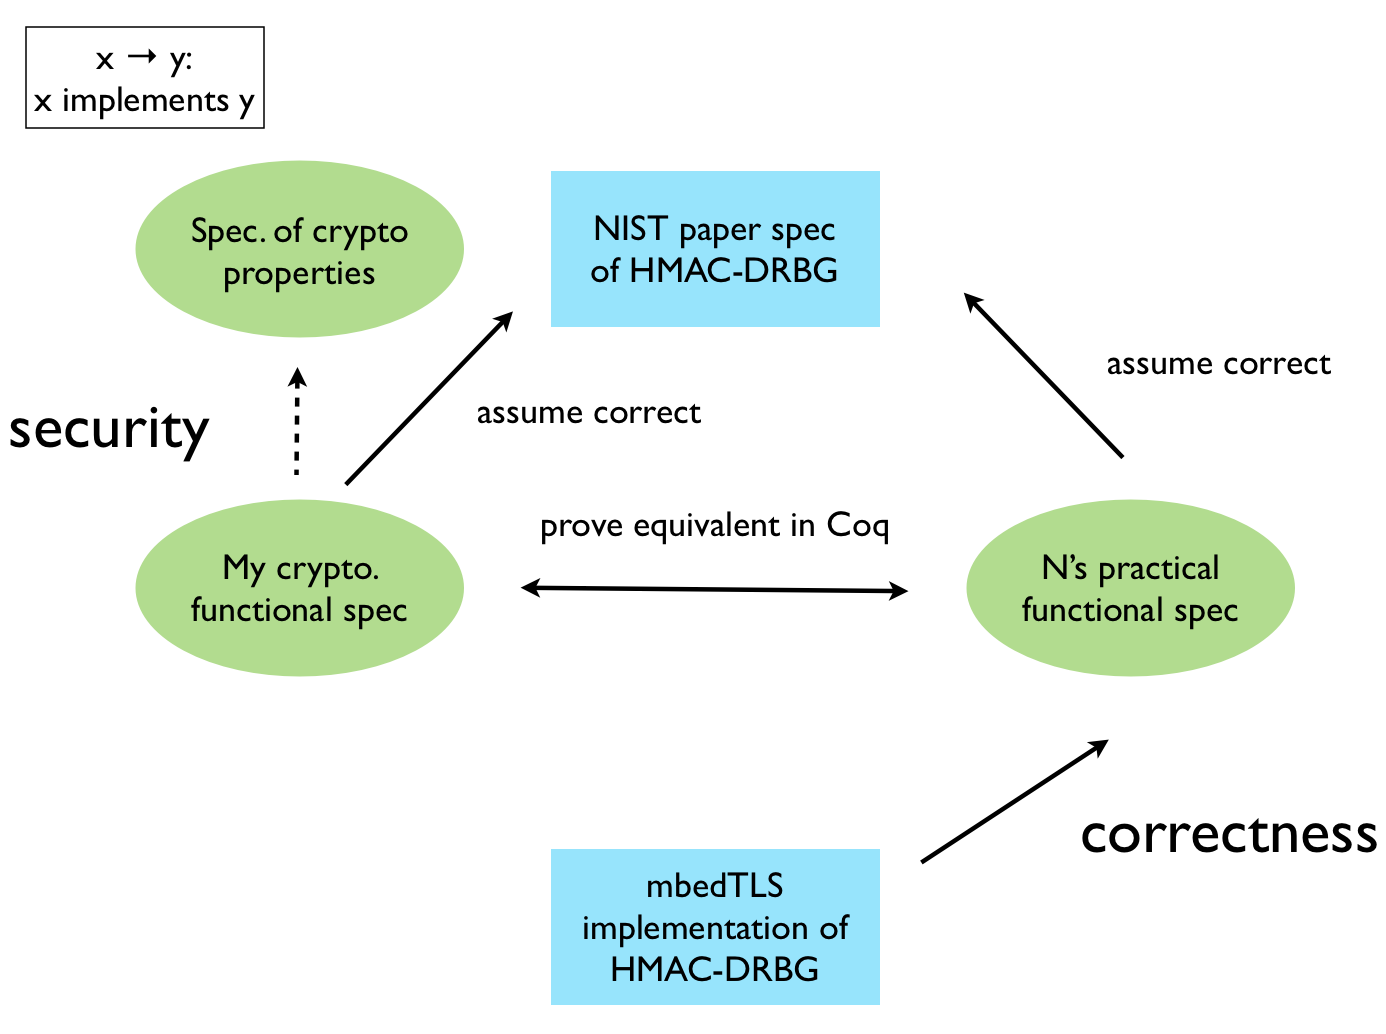
\includegraphics[width=\linewidth]{images/project_diagram.png}
  \caption{A fully verified HMAC-DRBG.}
  \label{fig:project_diagram}
\end{figure}

\subsection{Proving functional correctness of HMAC-DRBG}

To add: 
\begin{itemize}
\item VST overview. 
\item Hoare logic overview. 
\item Summary of Naphat's proof. 
\item A diagram of the whole project, similar to the HMAC diagram. 
\item My prior work for HMAC.
\end{itemize}

\subsection{Bridging the gaps between the specifications}

We must prove lemmas about at least the following differences between the specifications.

\begin{enumerate}
\item Naphat's code has essentially the same core loop ($Gen\_loop$) and $Generate$ and $Update$ code. However, it's surrounded by many layers of error checking code, e.g. for \li|prediction_resistance_request|. We need to prove equivalence modulo error checking.
\item Naphat's code also models failures in the type for the entropy stream. It is an infinite stream of either bit or failure. Also, it is not necessarily ideal randomness. We need to relate FCF's sampling uniformly at random to this more realistic entropy model. Adam Petcher's thesis provides some theorems about the operational semantics of FCF that can help us with this.
\end{enumerate}

\section{Future work}

HMAC is slow. AES is fast. Thus, AES CTR-DRBG, which uses AES in CTR mode, is much more widely used in practice than HMAC-DRBG (e.g. Amazon uses AES CTR-DRBG). It would be practically useful to formally verify HMAC-DRBG, but also theoretically interesting. How do our proofs generalize? (Some things would be different; e.g. HMAC is assumed a PRF, and AES is assumed a pseudorandom permutation. Their respective DRBGs are slightly different as well. Some things would break; e.g. to refresh the key without a collision, NIST cannot length-extend the input.) Can we build a general framework for verifying DRBGs? How automated can it be? Is the concrete security bound better?

All of this effort was predicated on the fact that HMAC-DRBG's specification will not change, and mbedTLS's implementation of HMAC-DRBG does not change. TODO: how modular are our proofs?

Also, OpenSSL's team is picking or designing a new PRNG (TODO correct this)--we hope our work encourages implementors to co-design with formal methods researchers.

\section{Conclusion}

We have contributed a paper proof of the pseudorandomness of a simplified version of HMAC-DRBG. Hirose (2008) had already written paper proofs, but they were complicated and not linked to functional specifications or implementations. No prior proof considered real-world use of HMAC-DRBG (or any similar DRBG) over multiple calls to the Generate function, or including updating of the state. Also, no prior proof has proven backtracking resistance for this type of DRBG.

We have mostly formally verified the pseudorandomness of a simplified version of HMAC-DRBG. Simple PRGs have been verified before, but they were on the order of verifying the core loop in $Generate$ (e.g. in the EasyCrypt documentation), not real-world PRGs.

We have contributed knowledge about the challenges and benefits of formally verifying PRGs, and especially about proving things about hybrid arguments. The process of writing a machine-checked proof of security unearthed several subtle errors, such as off-by-one errors in hybrid numbering and the presence of multiple PRF adversaries.

We plan to link this security proof to a functional correctness proof. Thus, mbedTLS's implementation of HMAC-DRBG will be fully certified.

%%%%%%%%%%%%%%%%%%%%%%%%%%%%%%%%%%%%%%%%%%%%%%%%%%%

\section{Acknowledgments}

I'd like to thank the following people for their help.

Adam Petcher provided a lot of help by walking me through using FCF, doing the proof of security for the core loop of the PRG, and debugging many of my proofs via (lengthy) email.

Matt Green came up with the proof of security for the simplified HMAC-DRBG, asked many tough questions about the Coq development, and patiently walked me through the crypto math. 

Andrew Appel provided lots of help with Coq proofs and suggestions for the future proof of equivalence. I'm glad he had the confidence that I would be able to do and verify crypto math (though it's not done yet!). Andrew has been a very active, supportive, and patient advisor during my JP, the grad school application process, and this thesis.

Lennart Beringer came to all of my thesis meetings and went above and beyond by helping me debug my proofs on Sundays.

Naphat Sanguansin did the work that would allow my proofs to actually hold on an implementation of HMAC-DRBG.

I want to thank Matt and Andrew again for suggesting a thesis topic that was cool and well-motivated, as well as providing detailed feedback on drafts of this thesis.

Thanks to everyone in 2D for general encouragement, cooking great food that sustained me at late hours, sending me thesis jams (thanks, Angela), and camping out with me in the dining room (hi, Jaehwan).

Thanks to Jean Juang, Frederic Koehler, and Xiaoyan Han for being great friends and thesis buddies, and Carolyn Chen and Pallavi Koppol for being great friends during the grad school application process.

Thanks to the Recurse Center for being a community of excellent people who are happy to listen to me ramble about research. 

% Signing out,\\
% \indent \it{Notorious P.R.G.}

%%%%%%%%%%%%%%%%%%%%%%%%%%%%%%%%%%%%%%%%%%%%%%%%%%%

% \section{References}

\bibliographystyle{plainnat}

\begin{thebibliography}{99}

\bibitem{affeldt2009}
Affeldt, Reynald, David Nowak, and Kiyoshi Yamada. "Certifying assembly with formal cryptographic proofs: the case of BBS." \emph{Electronic Communications of the EASST} 23 (2009).

\bibitem{appel2015}
Appel, Andrew W. "Verification of a cryptographic primitive: SHA-256." \emph{ACM Transactions on Programming Languages and Systems (TOPLAS)} 37, no. 2 (2015): 7.

\bibitem{barak2005}
Barak, Boaz, and Shai Halevi. ``A model and architecture for pseudo-random generation with applications to/dev/random.'' \emph{Proceedings of the 12th ACM conference on Computer and communications security.} ACM, 2005. 

\bibitem{barker2012}
Barker, Elaine, and John Kelsey. "NIST Special Publication 800-90A: Recommendation for random number generation using deterministic random bit generators." (2012).

\bibitem{barthe2011}
Barthe, Gilles, Benjamin Gr{\'e}goire, Sylvain Heraud, and Santiago Zanella-B{\'e}guelin. "Computer-aided security proofs for the working cryptographer." In \emph{Advances in Cryptology---CRYPTO} 2011, pp. 71-90. Springer Berlin Heidelberg, 2011.

\bibitem{barthe2014}
Barthe, Gilles, et al. ``Easycrypt: A tutorial.'' \emph{Foundations of Security Analysis and Design VII.} Springer International Publishing, 2014. 146-166.

\bibitem{bellare2004}
Bellare, Mihir, and Phillip Rogaway. "Code-Based Game-Playing Proofs and the Security of Triple Encryption." \emph{IACR Cryptology ePrint Archive} 2004 (2004): 331.

\bibitem{beringer2015}
Beringer, Lennart, Adam Petcher, Katherine Q. Ye, and Andrew W. Appel. "Verified correctness and security of OpenSSL HMAC." In \emph{24th USENIX Security Symposium (USENIX Security '15)}, pp. 207-221. 2015.

\bibitem{campagna2006}
Campagna, Matthew J. "Security Bounds for the NIST Codebook-based Deterministic Random Bit Generator." \emph{IACR Cryptology ePrint Archive 2006} (2006): 379.

\bibitem{dodis2013}
Dodis, Yevgeniy, David Pointcheval, Sylvain Ruhault, Damien Vergniaud, and Daniel Wichs. "Security analysis of pseudorandom number generators with input:/dev/random is not robust." In \emph{Proceedings of the 2013 ACM SIGSAC conference on Computer and Communications Security}, pp. 647-658. ACM, 2013.

\bibitem{dorre2015}
D{\"o}rre, Felix, and Vladimir Klebanov. "Pseudo-random Number Generator Verification: A Case Study." \emph{Proceedings, Verified Software: Theories, Tools, and Experiments (VSTTE)} (2015).

\bibitem{fouque2008}
Fouque, Pierre-Alain, David Pointcheval, and Sébastien Zimmer. ``HMAC is a randomness extractor and applications to TLS.'' \emph{Proceedings of the 2008 ACM symposium on Information, computer and communications security.} ACM, 2008.

\bibitem{goldreich2005}
Goldreich, Oded. \emph{Foundations of cryptography: a primer}. Vol. 1. Now Publishers Inc, 2005.

\bibitem{hirose2008}
Hirose, Shoichi. "Security analysis of DRBG using HMAC in NIST SP 800-90." In \emph{Information Security Applications}, pp. 278-291. Springer Berlin Heidelberg, 2008.

\bibitem{petcher2015}
Petcher, Adam, and Greg Morrisett. "The foundational cryptography framework." In \emph{Principles of Security and Trust}, pp. 53-72. Springer Berlin Heidelberg, 2015.

\bibitem{sanguansin2016}
Sanguansin, Naphat. "Verification of a Deterministic Random Bits Generator." Independent work paper, Princeton University. 2016.
\end{thebibliography}

%%%%%%%%%%%%%%%%%%%%%%%%%%%%%%%%%%%%%%%%%%%%%%%%%
 \appendix

\section{Definitions and proofs}

Will add worked examples of Coq proofs using FCF tactics. 

 \end{document}





























%%% Local Variables:
%%% mode: latex
%%% TeX-master: t
%%% End:
